%aa.dem
% AA vers. 9.1, LaTeX class for Astronomy & Astrophysics
% demonstration file
%                                                       (c) EDP Sciences
%-----------------------------------------------------------------------
%
%\documentclass[referee]{aa} % for a referee version
%\documentclass[onecolumn]{aa} % for a paper on 1 column  
%\documentclass[longauth]{aa} % for the long lists of affiliations 
%\documentclass[letter]{aa} % for the letters 
%\documentclass[bibyear]{aa} % if the references are not structured 
%                              according to the author-year natbib style

%

\documentclass{aa}  
\usepackage{booktabs}
\usepackage{amsmath}
\usepackage{amssymb}
\begin{document} 


\title{The peculiar nebula Simeis 57}

\subtitle{II. Distance, nature and excitation}

\author{L.H.T. Oudshoorn\inst{1}
      \and
      F.P. Israel\inst{1}
      \and
      J. Brinchmann\inst{1,2}
      \and
      M.B.C. Kloppenburg\inst{1,3}
      \and
      A.G.A. Brown\inst{1}
      \and
      J. Bally\inst{4}
      \and
      T.R. Gull\inst{5}
      \and 
      P.T. Boyd\inst{5}
      }
\let\oldAA\AA
\renewcommand{\AA}{\text{\normalfont\oldAA}}
\institute{Sterrewacht Leiden, P.O. Box 9513, 2300 RA Leiden, The Netherlands
     \and
         Instituto de Astrof\'isica e Ci\^encias do Espa\c{c}o, Universidade do Porto, CAUP, Rua das Estrellas, PT4150-762 Porto, Portugal
    \and
         Presently: Pels Rijcken, P.O Box 11756, 2502 AT Den Haag, The Netherlands
    \and 
        Center for Astrophysics and Space Astronomy (CASA), Univ. of Colorado, 389 UCB, Boulder, CO 808309, USA
    \and 
        NASA/GSFC, Mail Code: 667, Greenbelt, MD 20771, USA
    }

\date{Received ***; accepted ***}

% \abstract{}{}{}{}{} 
% 5 {} token are mandatory

\abstract
% context heading (optional)
% {} leave it empty if necessary  
{ Simeis~57 (HS~191) is an optically bright nebula in the Cygnus X
  region with a peculiar appearance that suggests an outflow from a
  rotating source. Newly obtained observations and archival data
  reveal Simeis~57 as a low-density ($n_{e}\,\sim\,100$ cm$^{-3}$)
  nebula with an east-to-west excitation gradient. The extinction of
  the nebula is $A_{V}\,\leq$ 2 mag.  The nebula is recognizable but
  not prominent in mid- and far-infrared images. In its direction,
  half a dozen small CO clouds have been identified at $V_{LSR}$ = + 5
  km s$^{-1}$. One of these coincides with both the optical nebula and
  a second CO cloud at the nebular velocity $V_{LSR}\,\approx$ -10 km
  $^{-1}$. No luminous stars are embedded in these molecular clouds,
  nor are any obscured by them and no sufficiently luminous stars are
  found in the immediate vicinity of the nebula. Instead, all
  available data point at the {\bf evolved HD~193793 = WR~140 (an O4-5
  supergiant and WC7 Wolf-Rayet binary)} as the exciting source,
  notwithstanding its large separation of $50'$ (about 25 pc at the
  stellar distance of 1.7 kpc). Simeis~57 appears to be a part of a
  larger structure surrounding the HI void centered on HD~193793.  }



   \keywords{Simeis 57 --
             DWB 111 --
             Propeller nebula --
             HD~193793 --
             WR~140 --
             ISM excitation
             }

   \maketitle
%
%-------------------------------------------------------------------

\section{Introduction}
The Galactic nebula Simeis~57, also known as HS~191 (\citet{Gaze1951},
\citet{Gaze1955}) is a very bright emission nebula of peculiar shape
in the constellation of Cygnus \citep[cf. ][]{Parker1979}. Often
referred to as the Propeller Nebula, it is a popular object for
amateur astro-photographers. Its major features are two curved
nebulosities (DWB~111 and DWB~119, Dickel et al. 1969). Its center is
cut by a long dust filament that continues adjacent to the nebular
patch DWB~118. More nebular emission may be part of the same complex.
This includes DWB~126 immediately to the north, as well as DWB~108 and
DWB~107 to the south. The brighter DWB~107, immediately southeast of
the nebula, has the appearance of a bright rim. At a Galactic
longitude of $80.3^{\circ}$, Simeis~57 is inside the Solar Circle but
its actual distance is unknown. In this direction Galactic sightlines
travel along the tangential part of the Orion-Cygnus spiral arm and
are several kiloparsecs long. However, the relatively high Galactic
latitude of $+4.7^{\circ}$ and the large angular extent ($\sim20'$)
suggest that it is not very distant.

Simeis~57 is located near the edge of a large
($18^{\circ}\times13^{\circ}$) X-ray structure known as the Cygnus
superbubble \citep{cash1980} but none of the X-ray or radio
continuum maps presented by \citet{uyaniker2001} shows anything
remarkable at its position, whereas the superbubble may not even be
a physical entity but merely a projection effect. Simeis~57 is well
away from the nearest OB associations (Cyg OB2 and Cyg OB8 at
heliocentric distances of 1.4 kpc and 1.8 kpc).

In an earlier paper, \citet{israel2003} presented high-resolution radio
continuum maps from which they concluded that the radio emission of
Simeis~57 is free-free thermal emission originating in a gas of
moderate electron densities ($<n_e^2>^{1/2}\sim100\, \mathrm{cm^{-3}}$
for an assumed distance of 0.5 kpc). They measured a
distance-independent emission measure $EM\,\approx\,5\times10^{3}$ pc
cm$^{-6}$. The comparison of the radio maps with low-resolution
H$\alpha$ emission established that the nebula suffers a modest
foreground extinction. The thermal radio emission, the limited
distance, and the low extinction suggest excitation by a star bright
enough to be easily identified. However, the lack of an obvious
candidate meant that the nature of Simeis~57 was left as a mystery.


% Figure 1: Ha large field overview
\begin{figure}
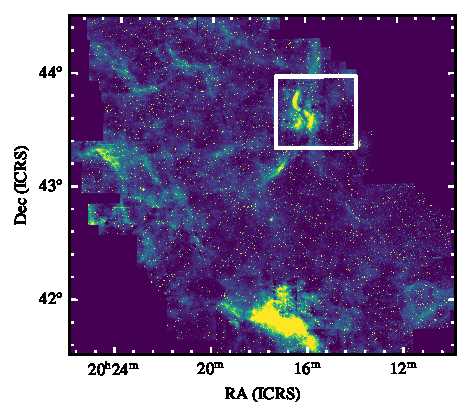
\includegraphics[width=0.48\textwidth]{Ha_largeregion_image.pdf}
\centering
\caption{Mosaic of H$\alpha$ line emission map of the surrounding
  $3^{o} \times 3^{o}$ region of Simeis~57 centered on
  $\alpha=20^{h}17^m50.4^s$, $\delta=+43^{\circ}01'48"$. The white box
  indicates the region studied in this paper, enlarged in
  Fig.\ref{fig:Ha_overview}}
\label{fig:Ha_mosaic}
\end{figure}

Here, we investigate the ionized gas, the dust, and the stars in the
field of Simeis~57 in a further attempt to identify its nature and the
source of its excitation. Fig.\,\ref{fig:Ha_mosaic} shows part of the
{\it Isaac Newton Telescope} Photometric H-Alpha Survey 
\citep[IPHAS, ][]{iphas1} combined with our own H$\alpha$ data described
below. It reveals many filaments at the outskirts of the Cygnus-X
region, among which Simeis~57 stands out in both brightness and shape.
In Fig.\,\ref{fig:Ha_overview}, we show the subdivision of the nebula
into four regions A, B, C, and D following \cite{israel2003}. Within
the smoothed $F_{1420}=20\,\mathrm{mJy \, arcmin^{-2}}$ contour, these
regions respectively cover areas of 45, 30, 10 and 15
$\mathrm{arcmin}^2$. Regions A (DWB~111) and B (DWB~119) form the
S-shaped nebula, region C is a spur that extends northwards from
region B and region D (DWB~118) is a separate filament to the
southeast.


%Figure 2: Ha small field 1420 MHz overlay with ABCD identification

\begin{figure}
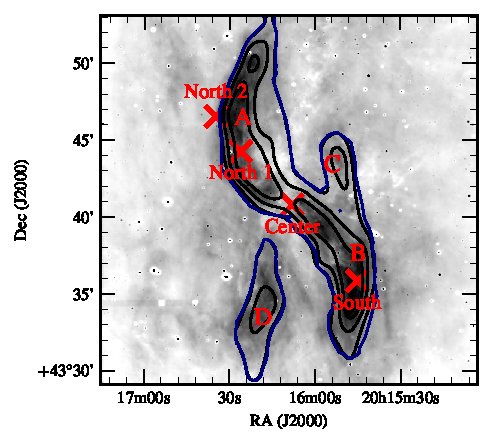
\includegraphics[width=0.48\textwidth]{Ha_overview.pdf}
\centering
\caption{The H$\alpha$ line emission map of Simeis 57 with
  the four subregions (A, B, C, D) described in the text, enclosed by
  the blue contour. Black contours correspond to DRAO 1420 MHz radio 
  continuum flux densities
  of 20, 25 and 30 $\mathrm{mJy \, arcmin^{-2}}$. Red crosses mark the
  central positions of the IDS long-slit spectra summarized in Table~1.}
\label{fig:Ha_overview}
\end{figure}


\section{Observations}


% Figure 3: spectra

\begin{figure*}
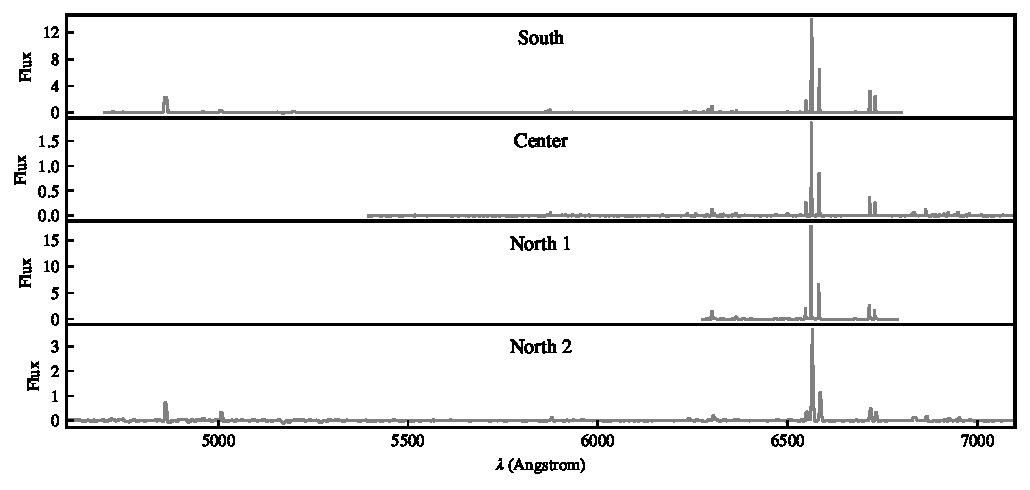
\includegraphics[width=0.98\textwidth]{Sim_INTspectra_NS.pdf}
\centering
\caption{Median collapsed long slit spectra for Simeis 57 at the
  positions marked in Fig.\,\ref{fig:Ha_overview}. Fluxes are in units
  of $10^{-16}\mathrm{erg\, cm^{-2} s^{-1}\AA^{-1}}$. }
\label{fig:spectra_3incol}
\end{figure*}

% Figure 4 Line images with radio contours

\begin{figure*}
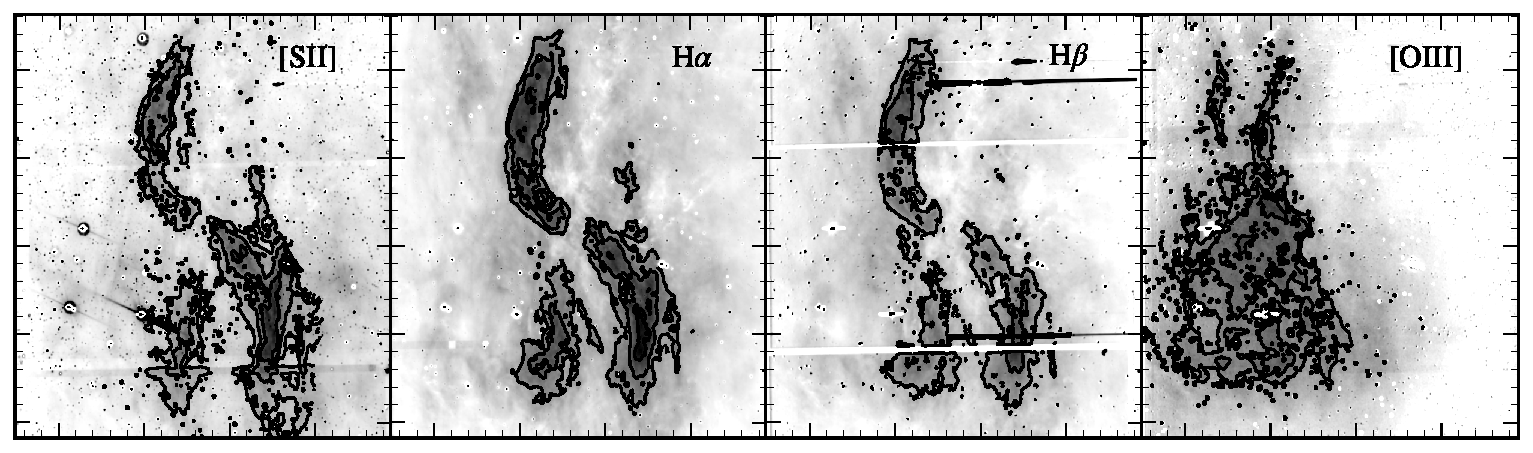
\includegraphics[width=0.98\textwidth]{line_images_simeis_4onrow.pdf}
\centering
\caption{Continuum-subtracted line images of the Galactic nebula
  Simeis 57 in identical fields of view. From left to right:
  [SII](6716+6730), H$\alpha$+[NII], H$\beta$ and [OIII]5007.  In
  each map, the first contour corresponds to
  $I_{\lambda} = (5.6, 18, 5, 1.4) \times 10^{-17}\, \mathrm{erg s^{-1}
  cm^{-2} \, arcsec^{-2}}$, respectively. In all maps, subsequent
  contours increase by factors of 1.5. The contours in the H$\alpha$
  +[NII] map represent the pure H$\alpha$ flux. The H$\beta$ image was 
  not dithered and therefore suffers from camera artefacts and gaps 
  between the CCDs.}
\label{fig:line_images_4onrow}
\end{figure*}


\subsection{Long-slit spectra}

We extracted archival spectra taken on July 22, 1990 and May 6, 2007 
and obtained new spectra on May 22-24, 2017 with the Intermediate Dispersion
Spectrograph (IDS) and the EEV10 detector on the INT. The INT is a
2.54m telescope located at the Observatorio del Roque de los Muchachos
on the island of La Palma (Spain). The IDS is a long-slit spectrograph
located at the Cassegrain focus, with a full unvignetted slit-length
of $3.3'$ and a spatial scale of $0.4"$/pix. In 2007 and 2017, we used
the R300V, R400V, and R600R gratings, with spectral resolutions of
$1.87$\AA/pix, $1.41$\AA/pix, and $0.94$\AA/pix, respectively and
wavelength ranges correspondingly decreasing. The 1990 spectrum used
Grating 10, which has a spectral resolution of $1.03$\AA/pix.
The spectra shown in Fig.\,\ref{fig:spectra_3incol} were taken at 
the positions listed in Table\,\ref{tab:observing_log_spectra} and 
marked in Fig.\,\ref{fig:Ha_overview}.


% Table 1:  Observations log

\begin{table}[h]
{\small %
\caption{Observing log of the INT-IDS spectroscopy.}
\label{tab:observing_log_spectra}
\begin{tabular}{lllllr}
\toprule
Grating    & Obs.       & RA J2000   & DEC J2000 &    & $T_{exp}$ \\
           & date       & hh:mm:ss.s &  dd:mm:ss &    & sec \\
\hline
R600R      & 2017-05-23 & 20:15:45.2 & +43:35:52 & S  & 600 \\
R400V      & 2017-05-25 & 20:15:45.2 & +43:35:52 & S  & 600 \\
R600R      & 2017-05-24 & 20:16:08.0 & +43:40:50 & C  & 600 \\
Gr.\,10    & 1990-07-22 & 20:16:26.1 & +43:44:18 & N1 & 4500\\
R300V      & 2007-05-06 & 20:16:35.0 & +43:46:34 & N2 & 300 \\
  \hline
\end{tabular}
} %
\end{table}

\par They were reduced with standard IRAF tasks for long-slit
reduction. Wavelength solutions were derived from arc lamp spectra and
cosmic rays were removed with the L.A.Cosmic package by
\cite{2012ascl.soft07005V}. For the flux calibration of the spectra
obtained in 2017 we used the standard star SP1550$+$330. The R300V
grating spectrum was calibrated with the standard star Kopff27. The
spectra shown in Fig.\,\ref{fig:spectra_3incol} are spatially
integrated over the aperture, excluding the outer 25 pixels on either
side. The two spectra taken at the southern position are concatenated
to yield a single spectrum. The northernmost spectrum was obtained
at the edge of DWB~111.




\subsection{WFC Images}

We obtained several images of Simeis~57, shown in
Fig.\,\ref{fig:line_images_4onrow}, in 2016 April and 2017 April with
the Wide-Field Camera (WFC) at the prime focus of the Isaac Newton
telescope (INT).  With four CCDs (thinned EEV) having
$2048\times 4096$ pixels each, the WFC is a mosaic camera operating at
optical wavelengths. The CCD pixel scale is $0.33"$ and the field of
view is $34.2'\times34.2'$.  Inter-chip gaps are about $1'$ in size.

\par We used the standard INT narrow-band filters (H$\alpha$, FWHM
$95\mathrm{\AA}$); [SII](6716+6730), $80\mathrm{\AA}$; H$\beta$
$30\mathrm{\AA}$; [OIII]5007, $100\mathrm{\AA}$, and broad-band
filters ($R$, FWHM $1347\mathrm{\AA}$); $G$, FWHM $1285\mathrm{\AA}$.
The narrow-band filters were used to trace the line emission from the
nebula and the broad-band filters to image the stars and sky.

\par We made multiple exposures in each filter. In 2017, we applied a
random dither of a few arcmin when taking the [SII] and [OIII] images
in order to fill the inter-chip gaps.  No dithering was applied to the
H$\alpha$ and H$\beta$ images that were both obtained in 2016. We
filled in the inter-chip gaps of the H$\alpha$ map by combining our
own five H$\alpha$ images with multiple exposures from the IPHAS
H$\alpha$ survey \citep{iphas1}. Total exposure times varied from
850 s for $R$ to 6400 s for [OIII]5007. Most lines were exposed for
about 3000 s. The average seeing of our observations is $1.7''$,
with the exception of H$\beta$ ($2.3''$) and H$\alpha$ ($1.3''$).

\par Individual exposures were debiased, flat-fielded and combined
using THELI \citep{SchirmerTheli,ErbenTheli}. Observations were made
during bright moon and suffered from significant sky brightness. We
estimated sky levels by taking the median of selected regions outside
the nebula after masking objects using SExtractor
\citep{1996A&AS..117..393B}.  We computed astrometric solutions using
SCAMP \citep{2006ASPC..351..112B} with the Gaia DR2 catalogue (see
Sect. 2.4). The astrometry should be better than 0.5$"$.

\par No spectro-photometric calibration stars were recorded during the
observations. Instead, H$\alpha$ and $r$ images are directly
calibrated with data from the INT/WFC Photometric H$\alpha$ survey of
the Northern Milky Way \citep[IPHAS DR2][]{iphas1} release, which was
made with the same instrument. This dataset has $i$, $r$ and H$\alpha$
magnitudes for nearly 5000 objects in our field of view. Using
SExtractor, we extracted magnitudes of all sources with S/N$\geq7$. We
used aperture photometry with the same diameter as the IPHAS database
($2.3"$, or 7 pixels). Local background subtraction was done
with a rectangular mesh of 16 pixels around the star. The magnitude 
zero-points have errors less than 0.15 mag in $r$ and H$\alpha$, 
caused mainly by small sky differences between different nights and images.

\par No calibrators or reference catalogues are available for the
continuum-subtracted [SII], [OIII] and H$\beta$ images. Instead, we
determined the relative-to-absolute flux conversion factors of the
images using the calibrated fluxes from the spectra in 
Fig.\,\ref{fig:spectra_3incol} sampled at four positions. For H$\alpha$, 
the two methods are consistent within $20\%$.

% Figure 5: Simeis 57 fields from UV to FIR

\begin{figure*}
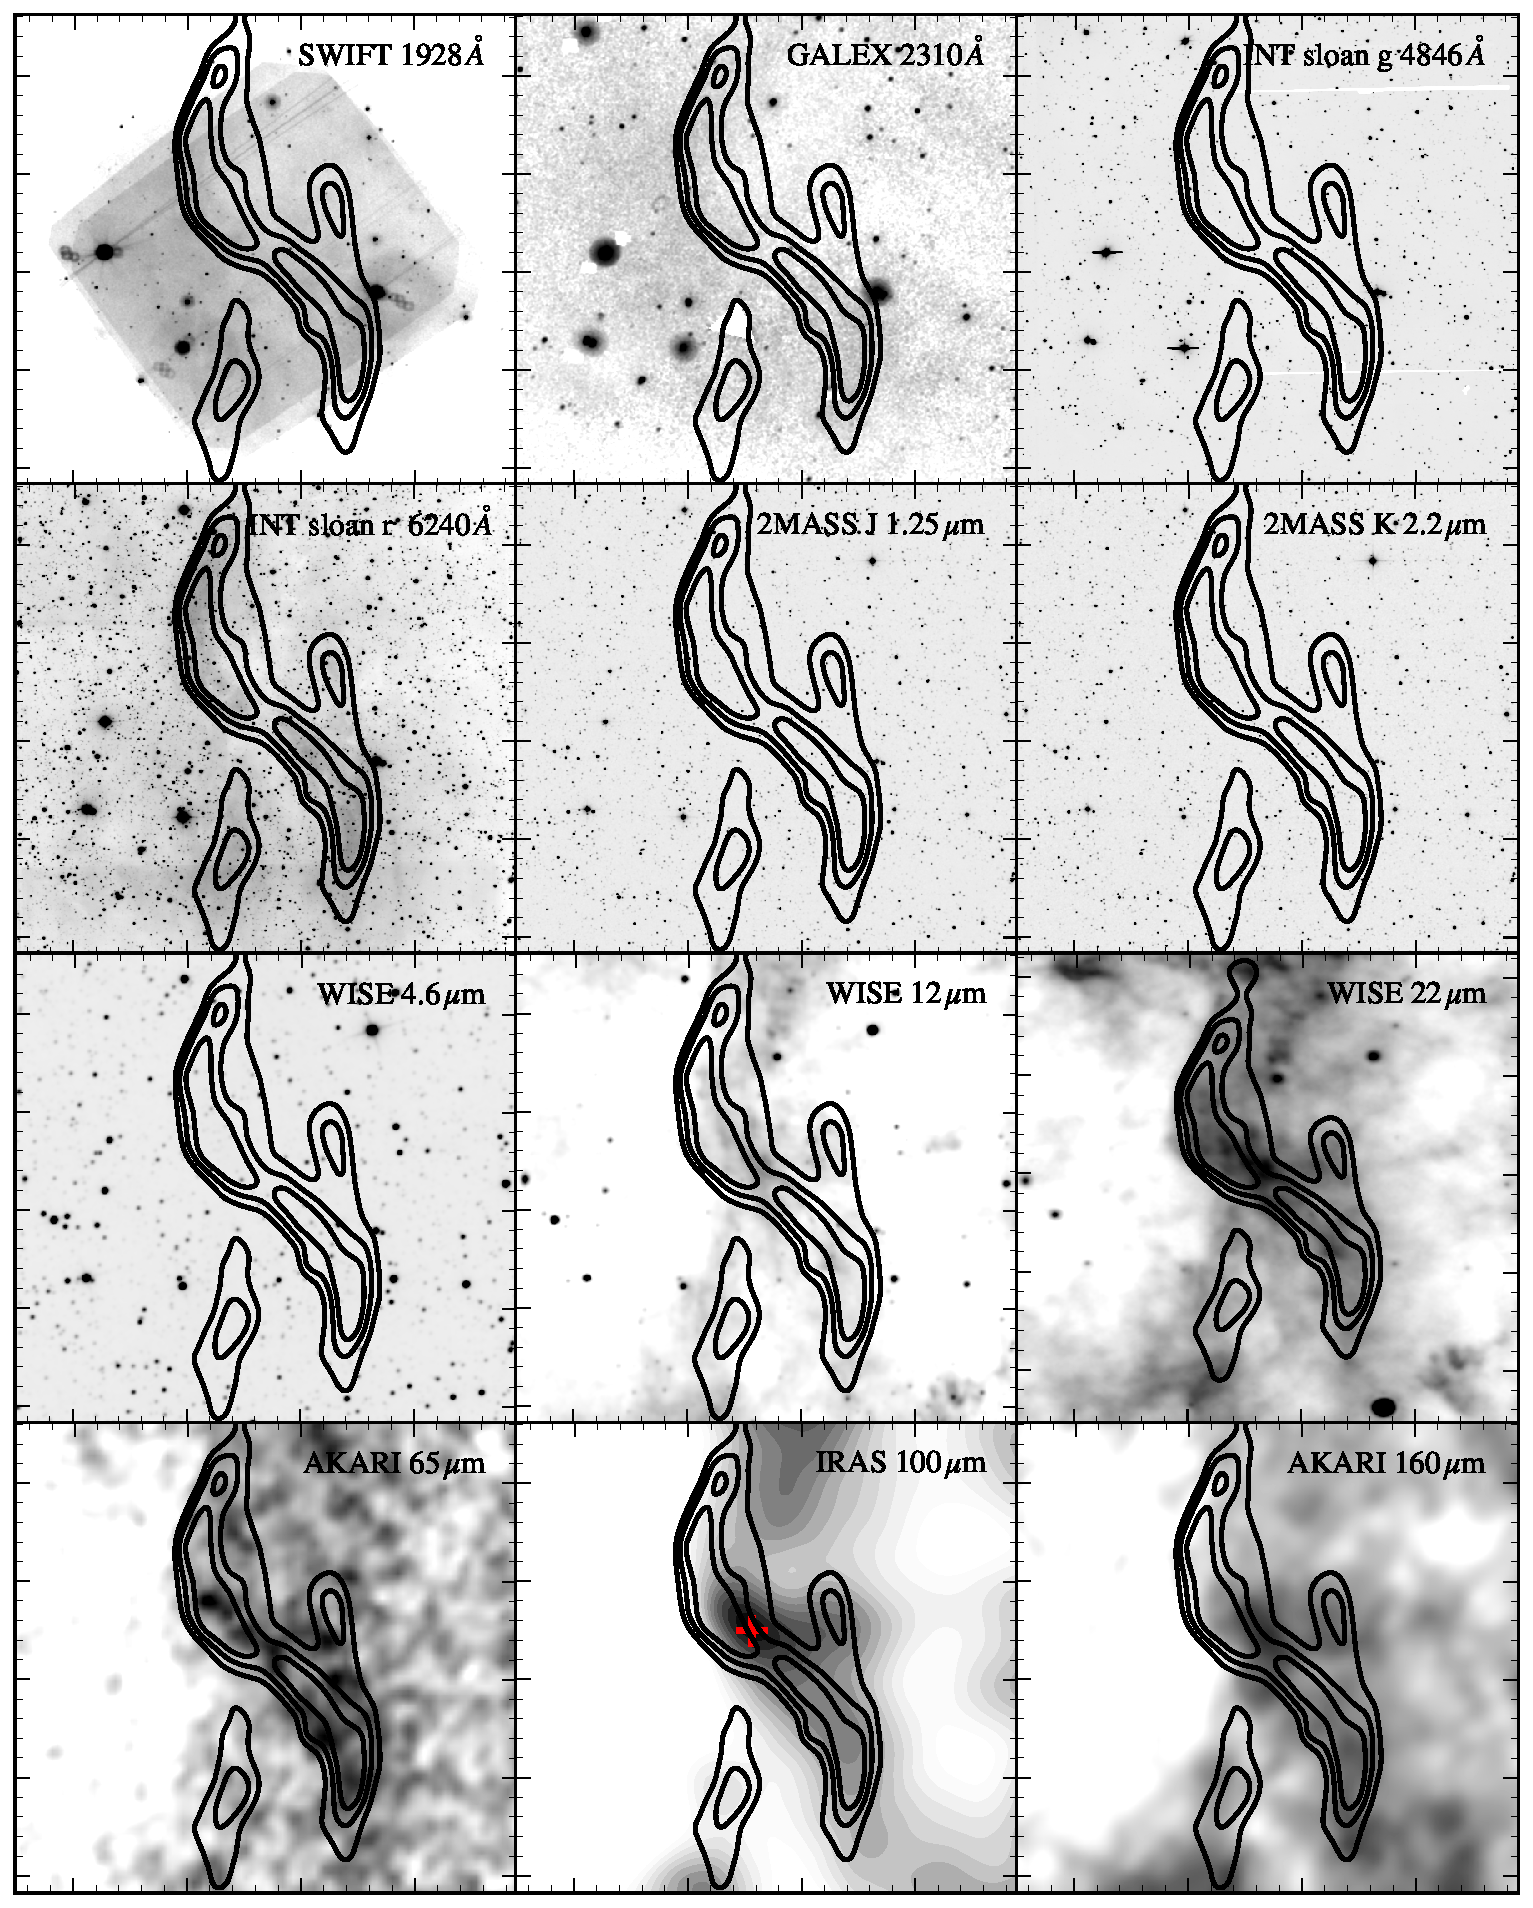
\includegraphics[width=0.92\textwidth]{ImageSpectrumSimeis_AKARI65.pdf}
\centering
\caption{UV, optical and infrared images of Simeis 57.  UV images are
  SWIFT UVOT ($\lambda_{eff} = 1928 \, \mathrm{\AA}$) and GALEX
  near-UV ($\lambda_{eff} = 2310 \, \mathrm{\AA}$) exposures. 
  Each image shows the same region of $0.4\times 0.4\,\mathrm{deg}$
  centered on $\alpha=304.04$, $\delta=43.69$. Optical broadband 
  images include those from our INT WFC observations with
  the filters sloan $g$ ($\lambda_{0} = 4846 \, \mathrm{\AA}$) and
  sloan $r$ ($\lambda_{0} = 6240 \, \mathrm{\AA}$).  Near-infrared
  images are 2MASS J and Ks band at wavelengths of 1.25
  $\mathrm{\mu m}$ and 2.2 $\mathrm{\mu m}$ and WISE band 2 to 4
  images, corresponding to wavelengths of 4.6, 12 and 22
  $\mathrm{\mu m}$.  Far-infrared images are AKARI 65, enhanced IRAS
  100 and AKARI 160 $\mathrm{\mu m}$.  The point source IRAS
  20145+4333 is marked by a red cross in the HIRES $100 \mathrm{\mu m}$
  map. Contours correspond to DRAO 1420MHz radio continuum
  intensities at 20, 25, 30 $\mathrm{mJy \, arcmin^{-2}}$.}
\label{fig:image_spectrum}
\end{figure*}


% Figure 6

\begin{figure*}
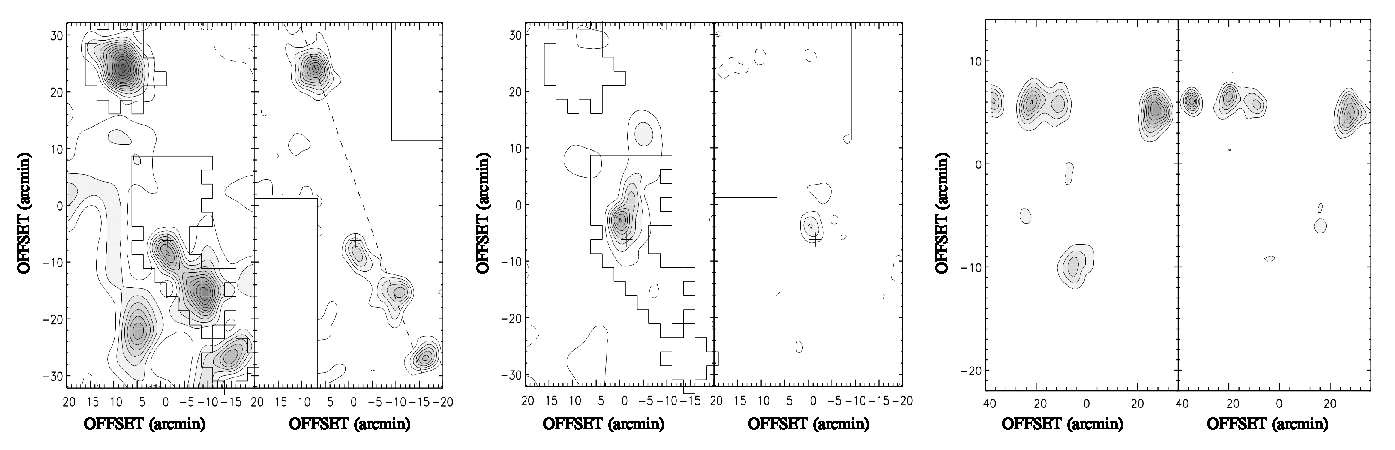
\includegraphics[width=1\textwidth]{BLT_CO.pdf}
\caption{Undersampled $J$=1-0 $^{12}$CO (left panels) and $^{13}$CO
  (right panels) maps of molecular clouds in the field of Simeis~57,
  whose center is marked by a cross. The emission at +5 km s$^{-1}$ is
  shown in the leftmost two panels (averaged over a 5 km s$^{-1}$
  velocity interval), and the central two panels show the emission at
  -10 km s$^{-1}$ (averaged over a 4 km s$^{-1}$ interval). In the
  $^{12}$CO panels, the regions with improved sampling are indicated
  by a solid-line boundary.  The rightmost two panels show the
  position-velocity map along the dashed line in the $^{13}$CO
  map. Position offsets are relative to $\alpha\,=\,20^h16^m16.7^s$,
  $\delta\,=\,+43^{\circ}47'54"$ (J=2000)}
\label{fig:blt_co_maps}
\end{figure*}

\subsection{UV data: Swift and GALEX}

% Figure 7: JCMT CO maps

\begin{figure*}
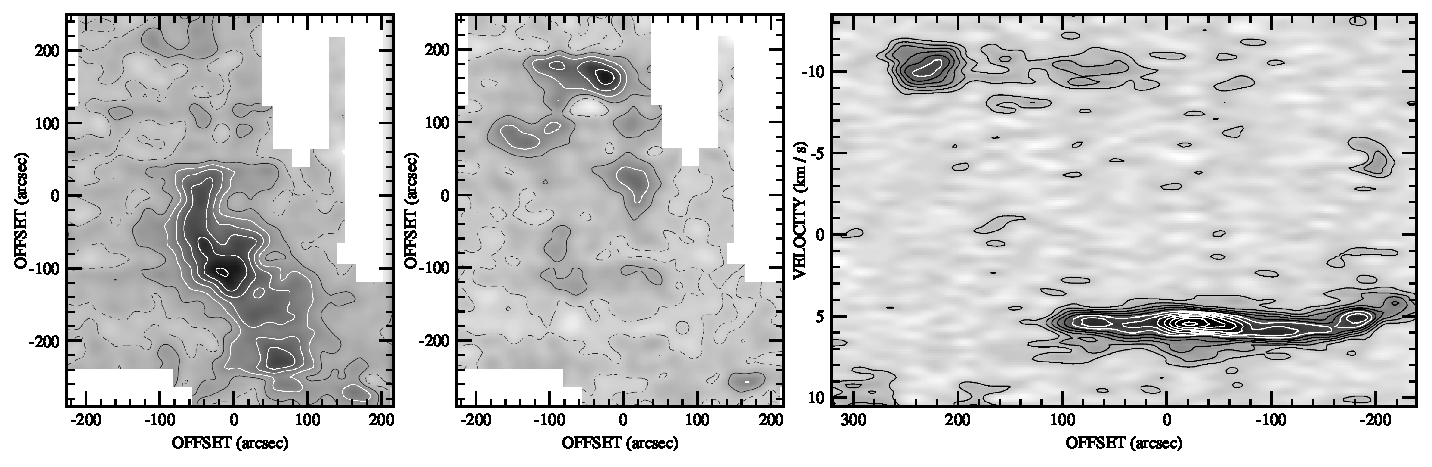
\includegraphics[width=1\textwidth]{COred_COblue_PV.pdf}
\centering
\caption{Fully sampled $J$=2-1 $^{13}$CO maps in the field centered on
  Simeis~57 (offset relative to $\alpha=20^h16^m08.2^s$,
  $\delta=43^{\circ}41'02.4''$) smoothed to a resolution of $30"$. At
  left is the emission at +5 km s$^{-1}$ (averaged over a 6 km
  s$^{-1}$ velocity interval), in the center the emission at -10 km
  s$^{-1}$ (averaged over a 10 km s$^{-1}$ interval), and at right the
  position-velocity distribution.}
\label{fig:jcmt_co_maps}
\end{figure*}

We obtained a UV image of the Simeis~57 field with the Neil Gehrels
Swift Observatory, {\bf a multi-wavelength space observatory launched
  in 2004. The on-board} Ultraviolet/Optical Telescope (UVOT) is a
modified Ritchey-Chr\'etien telescope with an aperture of 30 cm and an
f/2.0 primary re-imaged to f/13. {\bf Its 2048$\times$2048 pixel
  detection array combines a pixel scale of $0.5"$ with} a
  $17'\times17'$ field of view \citep{2008MNRAS.383..627P}. The
  observations were made between 2012 March and 2013 January in the
  UVW2 filter which has a maximum efficiency at
  $\lambda_{center} = 2000\mathrm{\AA}$.  At this wavelength, the
  resolution is about $1.5"$.

\par We also retrieved near-UV
($\lambda_{eff} = 2310 \, \mathrm{\AA}$) observations of the region
surrounding DWB~111 from the {\bf archive of the NASA GALEX space
observatory that operated 2003-2012. It was} equipped with a 50 cm
aperture telescope in a Ritchey-Chr\'etien f/6 configuration. It could
detect UV radiation between wavelengths of 135 nm to 280 nm with a
field of view of 1.2 degrees wide. We used MOSAIX
\citep{armengot2014mosaix} to stack the retrieved images.  In
Fig.\,\ref{fig:image_spectrum} we show both UV images.



\subsection{Optical data: Gaia}

Gaia \citep{refId0} is an ESA space observatory, launched in 2013.
Gaia uses two telescopes to perform astrometry,
photometry, and spectrometry of stars with very high precision down to
a visual magnitude of 20. In the absence of visual extinction, it
should thus see OB stars across the entire Galaxy. It was designed to
provide position, parallax, and annual proper motion with accuracies
of $0.025$ mas at $V$ -15 mag to $0.6$ mas at $V$=20 mag, and
distances accurate to $\leq1\%$, and $\leq10\%$, respectively.

\par From the second data release (DR2) in 2018, we extracted 218136
stars within a radius of one degree from the nebula and selected the
13381 stars ($6\%$) with high-quality data (RUWE $<$ 1.40) shown in
Fig.\,\ref{fig:gaia_figs}. Because stars associated with the
ionization of Simeis 57 should be hot, we {\bf specifically considered}
the 49 bright, blue stars with $M_{\rm G}\,<\,3$ and
$G_{\rm BP}-G_{\rm RP}\,<\,0.4$.  This sample defines the peak of the
main-sequence region in the HR diagram of the Simeis 57 region. Many
of the bright blue stars are visible in the NASA GALEX and ESO
Digitized Sky Survey (DSS2) data, and this includes a few close to the
propeller nebula itself.


\subsection{Infrared data: IRAS, 2MASS, WISE, Akari}
  
In order to investigate the infrared properties of Simeis~57 and
surroundings, we used the public databases kept at the NASA/IPAC
Infrared Science Archive (IRSA).  Far-infrared maps were constructed
from the {\it IRAS} and the {\it Akari} data, near- and mid-infrared
maps from the {\it WISE} data, and near-infrared maps from the {\it
  2MASS} data.

\par We used enhanced resolution {\it IRAS} \citep{Neugebauer_IRAS}
infrared continuum maps at 12, 25, 60 and 100 $\mathrm{\mu m}$ from
the Infrared Processing and Analysis Center (IPAC). The {\bf HIRES
  enhancements employs the Maximum Correlation Method (MCM)
  \citep{Aumann1990} in 20 iterations to construct
resolution-enhanced coadded {\it IRAS} images. The original {\it IRAS}
resolutions vary between $0.5'$ at 12 $\mathrm{\mu m}$ to about $2'$
at 100 $\mathrm{\mu m}$.  HIRES provided a roughly five-fold increase
in resolution, but the actual resolution varies over the map.}
A tilted plane was fitted to the background and subtracted. The
{\it IRAS} map in Fig.\,\ref{fig:image_spectrum} is dominated by
diffuse extended emission from warm dust.

\par Between 1997 and 2001, the University of Massachussetts carried
out an all-sky survey in the near-infrared using $256\times256$-pixel
$J$ 1.25 $\mathrm{\mu m}$, $H$ 1.65 $\mathrm{\mu m}$, and $K_{s}$
2.17 $\mathrm{\mu m}$ band arrays on two automated 1.3 m telescopes
\citep{skrutskie2006two}. The digital {\it 2MASS} sky atlas resulting
from the survey has a resolution of $4"$ in each of the three bands.
We constructed the {\it 2MASS} mosaics using the Montage software
package. In Fig.\,\ref{fig:image_spectrum} we show the $J$ and $K_{S}$
band images centered on Simeis~57. These images do not show the
nebular or dust emission, and are dominated by the stars in the field.

\par The NASA Wide-Field Infrared Survey Explorer ({\it WISE})
conducted an all-sky survey between 2009 and 2011. {\bf We downloaded
  from the archives images with a field of view of $47'$ at a
  resolution of $6"$, in four bands at 3.4, 4.6, 12 and
  22$\mathrm{\mu m}$. The last two bands are similar to the lower two
  {\it IRAS} bands but have} a much higher sensitivity. The field
centered on Simeis~57 is shown for bands two to four in
Fig.\,\ref{fig:image_spectrum}.  The near-infrared (4.6
$\mathrm{\mu m}$) image is dominated by the stars in the field, but
the two mid-infrared (12 $\mathrm{\mu m}$ and 22 $\mathrm{\mu m}$)
images show emission from hot dust associated with the nebula. {\bf
  Unlike the {\it IRAS} images, these very sensitive {\it WISE}
  images} still show the brightest stars.

\par {\it Akari} was an infrared observatory developed by the Japan
Aerospace Exploration Agency (JAXA) with ESA participation. Between
2006 and 2007 it conducted an all-sky survey in four far-infrared
bands at 65, 90, 140, and 160 $\mathrm{\mu m}$ at resolutions of $1'$
to $1.5'$ provided by a 68.5 cm aperture telescope
\citep{AkariPaper}. This resolution is lower than that provided by
{\it 2MASS} and {\it WISE} and comparable to HIRES, with the advantage
of being constant across the field. The data were released in 2014 as
$6^{\circ}\times6^{\circ}$ FITS {\bf images covering the whole sky.}
In Fig\,\ref{fig:image_spectrum}, we show images centered on Simeis~57
at 65 and 160 $\mathrm{\mu m}$. {\bf Like the {\it IRAS} images, they}
are dominated by the diffuse thermal emission from warm dust.
 
 
 
\subsection{Millimeter-wave CO data: BTL, NRAO, JCMT}

Dense clouds of dust and gas may hide such stars from our view. The
nebula may be part of a much larger molecular cloud complex not seen
at optical or infrared wavelengths. In order to investigate these
possibilities, we used the Bell Telephone Laboratories (BTL) 7 m
offset Cassegrain telescope in New Jersey, to observe the $J$=1-0
$^{12}$ CO and the $^{13}$ CO transitions in frequency-switched
mode. At the observing frequencies of 110 GHz and 115 GHz, the antenna
had a clean Gaussian beam of 100$"$. The observing and reduction
techniques were identical to those described by \cite{Bally1987}.  In
the undersampled $40'\times64'$ CO map we identified five small clouds
at a velocity of $V_{LSR}\,\sim\,+5$ km s$^{-1}$.  On four of them we
increased the map sampling to a $2.5'$ grid and we also mapped them in
$^{13}$ CO. At the map center, another cloud occurs at $V_{LSR}$ = -10
km s$^{-1}$ (Fig.\,\ref{fig:blt_co_maps}). Additional $J$=1-0
$^{12}$CO and $^{13}$CO observations were made in September 1989 with
NRAO 12m telescope at a resolution of $55"$, yielding good
$^{12}$CO/$^{13}$CO isotopologue ratios at various positions in the
central cloud.  Finally, the central cloud was mapped in various
observing runs between 2002 and 2005 at a higher resolution of $22"$
in the J=2-1 transition with the James Clerk Maxwell Telescope (JCMT)
in Hawaii. The $^{13}$CO map covers an area $420"\times560"$ and is
fully sampled (grid spacing $5"$ - $10"$)
(Fig.\,\ref{fig:jcmt_co_maps}). In $^{12}$CO two smaller $10"$ grid
maps were obtained centered on offsets (0, +200$"$) and (-80$"$,
-30$"$), respectively.


\section{Analysis}

\subsection{Distance}

{\bf \cite{israel2003} suggested that Simeis~57 is relatively nearby,
  given its out-of-the-plane location. From low resolution H$\alpha$
  imaging, they also found the extinction in front of Simeis~57 to
  vary between $A_V$ = 1.0$^{m}$ and $A_V$ = 2.8$^{m}$ with a mean of
  2$^{m}$.  Recent work based on Gaia, Pan-STARRS 1 and 2MASS by
  \cite{2019arXiv190502734G} allows us to review in more detail the
  reddening E(g-r)\footnote{For an $R_{V}$ = 3.1 reddening law,
    $E(B-V)\,\sim0.981\,E(g-r)$ \citep[see][]{Schlafly2011}.} of field
  stars in the direction of Simeis~57 as a function of distance
  (Fig.\,\ref{fig:reddening_with_D}).  Steep increases in reddening
  mark the presence of dust sheets at $m- M = 10.5^{m}$ and $m- M=
  12^{m}$ that can be translated into distances of $1.3\pm0.1$ kpc
  and $2.5\pm0.2$ kpc, respectively. The reddening changes at these
  distances correspond to extinction jumps from $A_V$ = 1.0$^{m}$ to
  2.4$^{m}$ and $A_V$ = 2.5$^{m}$ to 3.6$^{m}$ suggesting a distance
  between 1.3 and 2.5 kpc for Simeis~57.}

\par The distribution of extinction and parallaxes of the Gaia sample
stars is shown in Fig.\,\ref{fig:gaia_figs} where colored dots mark
the bright blue stars mentioned earlier.  The parallax distribution
has a sharp edge at about 0.35 milli-arcsec.  This corresponds to a
distance of about 3 kpc and a height above the plane of 250
pc. Obviously, at that point the line of sight is clearing the Milky
Way disk, which marks 3 kpc as the upper limit to the distance of
Simeis~57. The subset of bright blue stars samples a relatively large
range of distances between 350 pc and 1500 pc but it is not evident
that these stars are associated with each other or that Simeis~57 is
related to any of them.  Although the evidence is still inconclusive,
we adopt for the moment a distance $D\,=\,1.5\pm0.5$ kpc for the
nebula.

% Figure 8: Reddening vs distance modulus

\begin{figure}
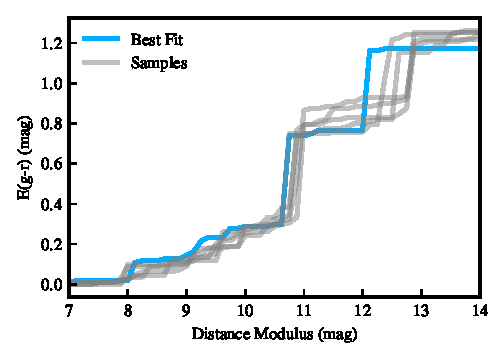
\includegraphics[width=0.48\textwidth]{Reddening_distance.pdf}
\centering
\caption{Reddening with distance based on \cite{2019arXiv190502734G}.
  Grey lines indicate stellar samples, the blue line marks the best
  model. }
\label{fig:reddening_with_D}
\end{figure}


%Figure 9: Gaia Figures

\begin{figure}
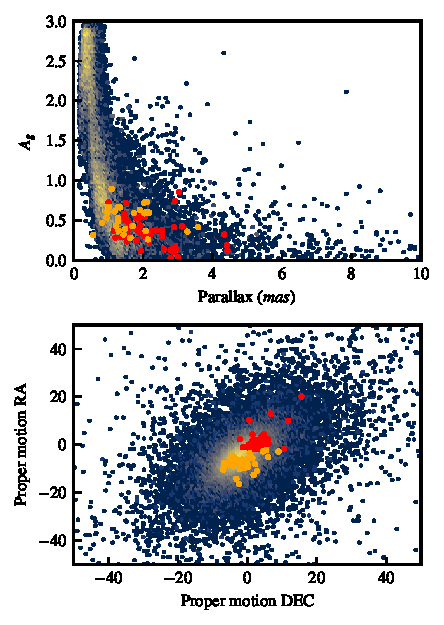
\includegraphics[width=0.48\textwidth]{GaiaResults.pdf}
\centering
\caption{Top: Gaia visual extinction ($A_g$ in mag) versus parallax
  (in milli-arcsec) for all stars with high-quality data within one
  degree of Simeis~57. Highlighted in this sample are 49 bright blue
  stars moving in predominantly NS (yellow dots) or EW (red dots)
  directions.  Bottom: Gaia proper motions for all stars within one
  degree of Simeis~57.  Red and yellow dots are the same as in the
  diagram at top.}
\label{fig:gaia_figs}
\end{figure}





\subsection{The nature of the nebular gas}


% Table 2: Spectral line ratios
\begin{table*}[ht]
{\small %
  \caption{Spectroscopic line ratios$^a$} 
  \label{tab:spectral_line_ratios}
\centering
\begin{tabular}{p{0.16\linewidth}p{0.14\linewidth}p{0.14\linewidth}p{0.14\linewidth}p{0.14\linewidth}}
\toprule
                        & North 2 & North 1 & Center & South \\
\midrule
Ha/[NII]        &  $2.2\pm0.08$ &  $2.0\pm0.19$ &  $1.9\pm0.21$ &  $1.7\pm0.12$ \\

Ha/[SII]        &  $4.1\pm0.12$ &  $3.8\pm0.14$ &  $3.2\pm0.27$ &  $2.5\pm0.11$ \\

\textbf{Ha/Hb}           &  $4.9\pm0.29$ &     $..$      &     $..$      &  $5.8\pm0.51$ \\

[NII] 6584/6548 &  $3.1\pm0.24$ &  $2.8\pm0.53$ &   $3.0\pm0.7$ &  $3.0\pm0.48$ \\

[NII] 6584/Ha   &  $0.3\pm0.01$ &  $0.4\pm0.02$ &  $0.4\pm0.04$ &  $0.4\pm0.02$ \\

[OIII]/Hb       &  $0.5\pm0.03$ &     $..$      &     $..$      &  $0.1\pm0.05$ \\

[SII] 6716/6731 &  $1.4\pm0.06$ &  $1.5\pm0.11$ &  $1.4\pm0.21$ &  $1.4\pm0.12$ \\

\bottomrule
\end{tabular}
\\
Note: a. Positions marked in Fig.\,\ref{fig:Ha_overview};
spectra shown in Fig.\,\ref{fig:spectra_3incol}.
b. [SII] and [NII] indicate the sum of the doublets.
} %
\end{table*}



\par Fig.\,\ref{fig:spectra_3incol} shows the spectra at the four
positions marked in Fig.\,\ref{fig:Ha_overview}. The [NII]6548\AA\,
and [NII]6584\AA\, lines flanking the H$\alpha$ line and the
[SII]6716, 6731\AA\, doublet are well-resolved. In all four spectra,
the relatively weak [OI]6300\AA\, and [OI]6334\AA\, lines can also be
made out. The former is about ten times weaker than H$\alpha$ and may
suffer from some atmospheric foreground contamination. Spectra
extending further into the visual, showing the H$\beta$4861\AA\, and
the [OIII]5007\AA\, lines, were obtained only at the southern and
northernmost positions. Line ratios are given in
Table\,\ref{tab:spectral_line_ratios}.  Similar spectra of the nearby Galactic HII region IC~1805 have
been discussed by \cite{Lagrois2012}.  Their diagnostic Figs. 12 and
13 imply that the Simeis~57 spectra are characteristic for the ionized
gas in an HII region at all positions.  The line ratios for the
southern position suggest a minor additional contribution by shocked
gas. The [NII]6584/6548\AA\, ratios $\sim3$ are consistent with the
[SII] doublet ratio of 1.4 that indicates low electron densities
$n_e\sim 30\, \mathrm{cm^{-3}}$ to $n_e\sim 100\, \mathrm{cm^{-3}}$ if
$T_e=10000\, \mathrm{K}$ \citep{2006agna.book.....O}. These electron
densities $n_e$ are very close to the r.m.s. electron densities
$<n_e^2>^{1/2}$ of about $60\pm15\, \mathrm{cm^{-3}}$ determined from
the radio maps by \cite{israel2003} adapted to $D$= 1.5 kpc, implying
clumping factors of about unity, i.e. a smooth ionized gas
distribution.

\par The nebular line images in Fig.\,\ref{fig:line_images_4onrow}
show similar distributions of ionized hydrogen (H$\alpha$, H$\beta$)
and ionized sulfur ([SII]). The peculiar `propeller' shape
of the nebula stands out, with a clear break in the middle apparently
caused by intervening dust (Fig.\,\ref{fig:line_images_4onrow}).

%Table 3: Line fluxes
%%%%BEGIN EDIT REFEREE
\begin{table}[h]
{\small %
  \caption{Area-integrated line fluxes}
  \label{tab:fluxes_info_from_maps}
\begin{center}
\begin{tabular}{lcccc}
\toprule
Region$^a$ & \multicolumn{4}{c}{Flux$^b$ ($10^{-11}\, \mathrm{erg\, cm^{-2}\,s^{-1})}$} \\
    &       [SII]  & H$\alpha^c$  &    H$\beta$  &  [OIII]        \\
\midrule
A   &   8.6 $\pm$ 2.1 &   30.8 $\pm$ 7.7 &  5.6 $\pm$ 1.4 &  1.7 $\pm$ 0.4 \\
A+B &  17.4 $\pm$ 4.3 &  57.9 $\pm$ 14.5 &  9.9 $\pm$ 2.5 &  2.5 $\pm$ 0.6 \\
B   &   8.8 $\pm$ 2.2 &   27.1 $\pm$ 6.8 &  4.3 $\pm$ 1.1 &  0.9 $\pm$ 0.2 \\
C   &   1.6 $\pm$ 0.4 &    5.2 $\pm$ 1.3 &  0.9 $\pm$ 0.2 &  0.2 $\pm$ 0.1 \\
D   &   3.2 $\pm$ 0.8 &   11.3 $\pm$ 2.8 &  2.0 $\pm$ 0.5 &  0.8 $\pm$ 0.2 \\
\bottomrule
  \end{tabular}
  \end{center}
Notes: a. Defined in Fig.\,\ref{fig:Ha_overview};
b. Continuum-subtracted, residual stellar emission masked;
c. Corrected for a $\sim35\%$ contribution by [NII] as suggested by
Fig.\,\ref{fig:spectra_3incol} and Table 2.
} %
\end{table}
%%%%END EDIT REFEREE
\par The [NII] doublet contributes significantly to the emission in the
H$\alpha$ filter. Taking our cue from the line spectra in
Fig\,\ref{fig:spectra_3incol}, we have corrected a constant [NII]
contribution of $35\%$ to the H$\alpha$ line emission measured in the
filter before constructing the [SII]-to-H$\alpha$ ratio map in
Fig\,\ref{fig:SII_over_Ha}. The variation across the map is
about $15\%$. Over most of the nebula, the [SII]/H$\alpha$ ratios are
close to 0.35, as expected for thermal emission from HII regions
\citep[cf. Fig. 12 from ][]{Lagrois2012}. Closer inspection of
Fig.\,\ref{fig:SII_over_Ha}, however, reveals ratios exceeding $0.4$ in
thin filaments or layers along the the western edges of both DWB~111
and DWB~119, higher than expected for pure thermal emission. They
provide evidence for the presence of shocks along the western edge of
Simeis~57, consistent with the line ratios in the southern
spectrum. Although the radio continuum spectral index map 
\citep[Fig. 7 of ][]{israel2003} does not show any trace of non-thermal
radio emission at these locations, this could reflect the
relatively poor resolution of that map.



% Figure 10: [SII] over Ha with radio contours

\begin{figure}
   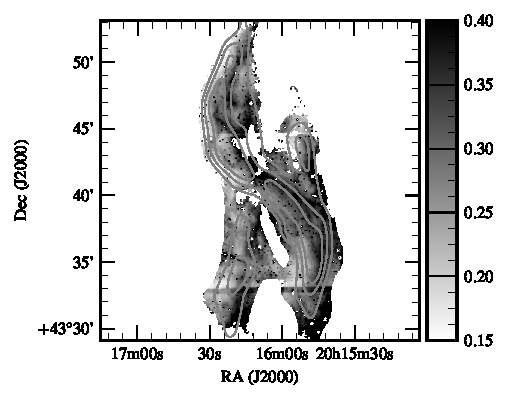
\includegraphics[width=0.48\textwidth]{SII_over_Ha.pdf}
 \centering
 \caption{
   Distribution of [SII]/H$\alpha$ line flux ratios. Only
   pixels with significant emission are included. The observed
   H$\alpha$ intensities have been corrected for a $35\%$ contribution
   from the nearby [NII] lines. Dark spots, gaps, and a horizontal bar
   are artefacts from different seeing conditions and the dithering
   procedure. Light grey contours are radio contours as in Fig. 
   \ref{fig:Ha_overview}.}
\label{fig:SII_over_Ha}
\end{figure}




\par The distribution of ionized oxygen ([OIII]) is very different
from that of the ionized hydrogen.  It shows a more diffuse nebula
and the propeller shape is not prominent.  In region A (DWB~111), the
[OIII] emission is mostly present in a thin ridge along the eastern
edge of the northern propeller `blade'. There is virtually no diffuse
[OIII] emission west of the propeller, and the extended diffuse oxygen
emission east of the propeller resembles only the weak, diffuse Balmer
line emission found there. The southern propeller 'blade' region B
(DWB~119) does not show up at all in [OIII] although it is bright in
the Balmer lines and in the radio continuum.

\par The ionized sulfur [SII] emission closely follows the Balmer line
emission, also across DWB~119.  It is prominent in the `spur' (region
C) northwest of the obscured center where no oxygen is seen. The
intensities of ionized sulfur [SII] and ionized oxygen [OIII] are
largely anti-correlated as essentially all sulfur is ionized up to
[SIII] or [SIV] in the [OIII] emitting zone.

\par The {\it WISE} mid-infrared images and especially the {\it IRAS}
and {\it Akari} far-infrared images likewise appear anti-correlated
with the [OIII] emission. They show diffuse extended emission west of
the propeller and a near-lack of infrared emission east of the nebula
where the [OIII] emission is prevalent. It appears that there is a
general lack of material in sight-lines east of Simeis~57 and that the
ionized gas at the eastern edges is much more highly excited than the
dusty gas to the west.


\subsection{Dust extinction towards Simeis~57}
%%%% BEGIN EDIT REFEREE
\par \textbf{To establish properties of Simeis~57 such as its
  H$\alpha$ luminosity, distance and source of ionization, we need to
  constrain the dust extinction towards Simeis~57. This can be done
  using the H$\alpha$ and H$\beta$ line and 1420 MHz continuum
  intensities. The nebular emission-line intensities and the color
  excess are related via \citep[see for details][]{Momcheva_2013}}
\begin{equation}
\begin{split}
    E(B-V) &= \frac{E(H\beta-H\alpha)}{k(\lambda_{H\beta})-k(\lambda_{H\alpha})}\\
    &= \frac{2.5}{k(\lambda_{H\beta})-k(\lambda_{H\alpha})} \log \Big[\frac{(H\alpha/H\beta)_{int}}{(H\alpha/H\beta)_{obs}} \Big]
\end{split}
\end{equation}
\noindent
\textbf{where $k(\lambda$ is the value of the reddening curve at the
  wavelength of $\lambda$.  $(H\alpha/H\beta)_{int}$ and
  $(H\alpha/H\beta)_{obs}$ are the unreddened and observed line
  ratios, respectively. In Table\, \ref{tab:fluxes_info_from_maps} we
  find for the latter about $5.8\pm2$.  The ratios of the map fluxes
  and the local values implied by the spectra in Table\,2 differ
  somewhat, reflecting nebular structure and calibration
  uncertainties. Assuming Case B recombination at
  $T_e=10000\,\mathrm{K}$ conditions \citep{2011piim.book.....D}, we
  expect (H$\alpha$/H$\beta$)$_{int}=$ 2.86. $E(H\beta-H\alpha)$ is
  analogous to $E(B-V)$ but defined for H$\beta$ and H$\alpha$. Using
  a standard Milky Way reddening law \citep{Cardelli1989} we find:}
\begin{equation}
\begin{split}
    E(H\beta - H\alpha) &= -2.50 \log \Big[\frac{(H\alpha/H\beta)_{int}}{(H\alpha/H\beta)_{obs}} \Big] = 0.77\pm0.37\\
    E(B-V) &= -1.97 \log \Big[\frac{(H\alpha/H\beta)_{int}}{(H\alpha/H\beta)_{obs}} \Big] = 0.60\pm 0.29
\end{split}
\end{equation}
\textbf{With}
\begin{equation}
    A_{\lambda} = k(\lambda) E(B-V)
    \label{eqk_lambda}
\end{equation}
\textbf{we obtain}
\begin{equation}
\begin{split}
    A_V \,&= 3.1\times E(B-V)=1.88\pm0.9\,\mathrm{mag}\\
    A_{H\alpha} &= 2.6\times E(B-V) = 1.6\pm0.8\,\mathrm{mag}    
\end{split}
\end{equation} 
\textbf{These extinction values are consistent with both the result
  obtained by \cite{israel2003} and the average Galactic visual
  extinction rate of 1.8$^{m}$ per kiloparsec 
  \citep{whittet2002dust}.}

\par The H$\alpha$ line and 1420 MHz radio continuum images are very
similar since the emission mechanisms are intimately related.  Unlike
the H$\alpha$ line, the emission at radio frequencies does not suffer
extinction and the intensity ratio of the two images allows a
derivation of the extinction across the entire nebula.  \textbf{In
  their earlier attempt, \cite{israel2003} used the relatively
  low-resolution VTSS H$\alpha$ survey to derive the extinction across
  the nebula. With the new H$\alpha$ image, we can improve the
  resolution of the extinction map by more than a factor of two. }
  %%%% END EDIT REFEREE
  The limiting factor is the resolution ($58"\times 80"$) of the 1420
  MHz DRAO radio continuum map.  For electron temperatures
  $T_e=10000 \, \mathrm{K}$, we expect optically thin free-free
  continuum and H$\alpha$ line emissivities
\begin{equation}
\begin{split}
    \epsilon_{1420} &= 3.9 \times 10^{-39} \, \mathrm{n_e^2 \, erg \, s^{-1} \, cm^{-3}\, Hz^{-1}}\\
    \epsilon_{H\alpha} &= 3.6 \times 10^{-25} \, \mathrm{n_e^2 \, erg \, s^{-1} \, cm^{-3}}
\end{split}
    \label{eq:opticallythin1420}
  \end{equation}
yielding an extinction-free ratio
\begin{equation}
     \frac{S_{1420}}{F(H\alpha)} = 1.15\times 10^{-14}\, \mathrm{Hz^{-1}}
    \label{eq:relation_radio_Ha}
  \end{equation}


  \noindent \textbf{that may be compared to observed ratios.} In the
  extinction map thus constructed (Fig.\,\ref{fig:co_extinction_map}),
  we have masked regions with
  $F_{1420}\leq 10\, \mathrm{mJy \,arcmin^{-2}}$ and assumed an
  extinction law $A(\lambda)\sim \lambda^{-1}$, so that
  $A_V \approx 1.2 A_{H\alpha}$.
\par In this map, the elongated extinction feature north of the center
of Simeis~57 coincides with part of the long radio filament mentioned
before. Its southern continuation has a radio counterpart (DBW~118;
region D) seemingly suffering only modest extinction. In fact, most of
the bright H$\alpha$ emission associated with the radio source suffers
relatively little extinction and is consistent with dust in the
foreground line of sight. The extinction in
Fig.\,\ref{fig:co_extinction_map} agrees well with the reddening implied
by the H$\alpha$/H$\beta$ line ratio, leaving little or no room for
the 'grey' extinction that would betray dust internal to the ionized
gas.  The absorption feature between the long radio filament and the
northern propeller 'blade', offset to the northeast from the center of
the nebula, has an infrared counterpart catalogued as IRAS PSC
20145+4333, marked in Fig.\,\ref{fig:image_spectrum} which appears
diffuse and resolved.  There is another well-defined extinction
feature west of and adjacent to region C (the spur).

%%%% START EDIT REFEREE
\par \textbf{Using the mean extinction $A_{H\alpha} $= 1.6$^{m}$, we
  convert the H$\alpha$ flux measured from region A+B in Table
  \ref{tab:fluxes_info_from_maps} into the intrinsic
  H$\alpha$ luminosity}
%as probed by the ratio of H$\alpha$ to H$\beta$ 
%($A_{H\alpha}\sim 2.3$) can be used to derive the H$\alpha$ 
%output of Simeis~57. Using the assumed distance of 
%$D\sim1500\,\mathrm{pc}$, the integrated
%H$\alpha$ luminosity is 
\begin{equation}
\begin{split}
    L_{H\alpha} &= 4\pi D^2 F_{H\alpha} 
    10^{\frac{A_{H\alpha}}{2.5}} \\
    &= (6.8\pm 1.6)\times 10^{35} \left(\frac{D}{1500\, pc}\right)^2\, 
    \mathrm{erg \, s^{-1}}
\end{split}
    \label{eq:Hafluxtoluminos}
\end{equation}
\textbf{For case B recombination, $T=10 000 \, \mathrm{K}$ and
  $n\sim 10^2\,\mathrm{cm^{-3}}$, the number of absorbed (stellar)
  Lyman continuum photons $N_{Lyc}$ is related to $L_{H\alpha}$ via
   \citep[cf.][]{Kennicutt:1994wu} }
%\begin{equation}
%    N_{L\gamma C} = \frac{H_{\beta}}{h c (j_{H\alpha}/j_{H\beta})} \frac{\alpha^{B}}{\alpha^{eff}_{H\beta}} L(H\alpha)  \, s^{-1}
%    \label{eq:LyafromHa}
%\end{equation}
%Where $j_{H\alpha}/j_{H\beta}$ is the intrinsic $H\alpha/H\beta$ line
%ratio, $\alpha^{B}$ the Case B recombination coefficient and 
%$\alpha^{eff}_{H\beta}$ the effective recombination coefficient for 
%the $H\beta$ line. Using $T=10 000 \, \mathrm{K}$ and 
%$n\sim 10^2\,\mathrm{cm^{-3}}$.
%, such that $j_{H\alpha}/j_{H\beta}=2.86$.
%We obtain the simplified relationship between H$\alpha$ luminosity
%and rate of absorbed L$\gamma$C photons
\begin{equation}
\begin{split}
    N_{L\gamma C} &=  7.1 \times 10^{11} L(H\alpha)\\
    &=(4.8\pm1.1)\times 10^{47}\, \left(\frac{D}{1500\, pc}\right)^2\, \mathrm{s^{-1}}
    \label{eq:LyafromHa}
\end{split}
\end{equation}

%%%% END EDIT REFEREE

\subsection{Infrared emission from dust}

\par The first emission from dust is seen in
Fig.\,\ref{fig:image_spectrum} at $12\,\mathrm{\mu\,m}$ and most 
of it appears to
be unrelated to the nebula, especially the emission north and south of
Simeis~57. The linear extinction feature separating DWB~111 (region A)
and DWB~119 (region B) is easily recognizable at mid-infrared
wavelengths of $12\,\mu$m and $25\,\mu$m but its far-infrared
counterpart is weak at best, suggesting that the emitting dust is
relatively warm. The propeller-shaped nebula is only traced at longer
wavelengths from $22\,\mathrm{\mu\, m}$ to $100\,\mathrm{\mu\, m}$. 
In the WISE $65\,\mathrm{\mu\, m}$
image, the emission from warm dust traces the northern DWB~111 'blade'
in the center, but the southern DWB~119 'blade' at the edge. The
compact dusty region IRAS 20145+4333 (marked in the IRAS 
$100\,\mathrm{\mu\, m}$ image) is indistinct in the 
$12\,\mathrm{\mu\, m}$ image but clearly present
longwards of $22\,\mathrm{\mu\, m}$. It does not confirm 
to the emission expected from an embedded stellar object.

\par Compared to other Galactic sources, the infrared emission from
Simeis~57 is insignificant. Unlike its optical counterpart, the object
does not stand out in infrared images at any wavelength.

We extracted the infrared brightnesses at the frequencies available
from the IRAS and AKARI databases, estimating the infrared background
from the empty region east of the object. We then derived the
(area-integrated) infrared fluxes of both the central compact object
IRAS 20145+4333 and the whole nebula
(Table\,\ref{table:IR_luminosities}).

% Table 4 Infrared luminosities

\begin{table}
\caption{Area-integrated infrared fluxes.}
   \label{table:IR_luminosities}
\begin{center}
\begin{tabular}{lrrcc}
\toprule
Mission& $\lambda$ & $\nu$ & Flux$^{a}$   & Flux$^{b}$    \\
       &($\mu$m)   & (THz) & (Jy)        & (Jy)          \\
\midrule
IRAS   &        12 &    25 &  13$\pm$4   &   56$\pm$42   \\
IRAS   &        25 &    12 &  35$\pm$7   &  136$\pm$83   \\
IRAS   &        60 &     5 & 326$\pm$67  & 1350$\pm$781  \\
AKARI  &        60 &     5 & 275$\pm$67  & 1265$\pm$657  \\
AKARI  &        90 &     3 & 251$\pm$18  & 1259$\pm$578  \\
IRAS   &       100 &     3 & 511$\pm$100 & 2368$\pm$1265 \\
AKARI  &       140 &     2 & 173$\pm$41  &  807$\pm$431  \\
\bottomrule
\end{tabular}
\end{center}
Notes: a. PSC IRAS 20145+4333, integrated over a solid angle of
$76\, \mathrm{arcmin^2}$.  b. Entire nebula, integrated over
a solid angle of $550\, \mathrm{arcmin^2}$.
\end{table}

The infrared luminosity of the compact region is only
$L_{\rm TIR}(compact)\,\approx\,1.5\times 10^{3}\times(D/1500
pc)^2\, \mathrm{L_{\odot}}$ \citep[using][]{Lee_1996}.
Its spectral shape matches that of an
embedded OB star \citep{wood1989massive} but the luminosity is
orders of magnitude below that expected for such a star. Even when 
integrated over the much larger area of $550\, \mathrm{arcmin^{2}}$, 
the infrared luminosity of the entire nebula remains low at
$L_{\rm TIR}(Si57)\,\approx 7\times 10^{3}\times(D/1500
pc)^2\,\mathrm{L_{\odot}}$. By fitting a
modified blackbody \citep{battersby2011characterizing} to the AKARI
and IRAS data with a $\beta=1.6$ emissivity to model dust temperatures 
we find $T_D \approx 36\, \mathrm{K}$.

At the nominal distance of 1.5 kpc, the found value of $L_{\rm TIR}$
corresponds to the luminosity of an embedded early-main-sequence B0.5
star with an absolute visual magnitude $M_V\,\approx\-2^m.8$
\citep{1973AJ.....78..929P}.  \textbf{This is only a minmum estimate
  as the radiating dust may subtend a solid angle
  substantially less than $4\pi$ as seen from the star.}
  For instance, if only $10\%$ of the sky were blocked by dust, an O7 star
  with $M_V\,=\,-4.2\, \mathrm{mag}$ would be needed, and with a
  blockage of only $1\%$ an O4/O5 star with
  $M_V\,=\,-5.8\, \mathrm{mag}$ would be required.  The analysis of
  the observed radio continuum or Balmer line emission leads to
  similar results.





\subsection{Molecular clouds and Simeis~57}

Our observations show surprisingly little CO emission towards Simeis
57. The nebula is associated with a molecular cloud smaller than the
optical nebula. The larger field lacks major molecular cloud
structures and instead contains a number of isolated small molecular
clouds in a narrow velocity range ($V_{LSR}$ = +4.4 to +6 km $^{-1}$)
Fig.\,\ref{fig:blt_co_maps}. The clouds, with sizes of 3 to 8 pc,
coincide with undistinguished far-infrared features
(Fig.\,\ref{fig:image_spectrum}). None of them shows clear signs of
external or internal heating, for instance by an embedded star.

\par \textbf{Peak line intensities are modest and line profilesare
  narrow (line widths 0.7 to 1.3 $\mathrm{km\,s^{-1}}$) characteristic
  of relatively cold, quiescent molecular gas. The $J$=1-0
  $^{12}$CO/$^{13}$CO isotopologue ratios $R_{10}$ range from
  $4.5\pm0.5$ to $7.0\pm0.8$. The small cloud at the center of
  Simeis~57 has a negative velocity $V_{LSR}$ = $-10.9$ km s$^{-1}$
  (cf. Fig.\,\ref{fig:blt_co_maps}), practically identical to the
  recombination line velocity of the ionized gas $V_{LSR}$ =
  $-12\, \mathrm{km\,s^{-1}}$ \citep{Pipenbrink1988}. Its isotopologue
  ratio is higher ($R_{10}$ = $11.0\pm0.3$ which suggests a lower CO
  optical depth.  }

% Figure 11 Extinction map

\begin{figure*}
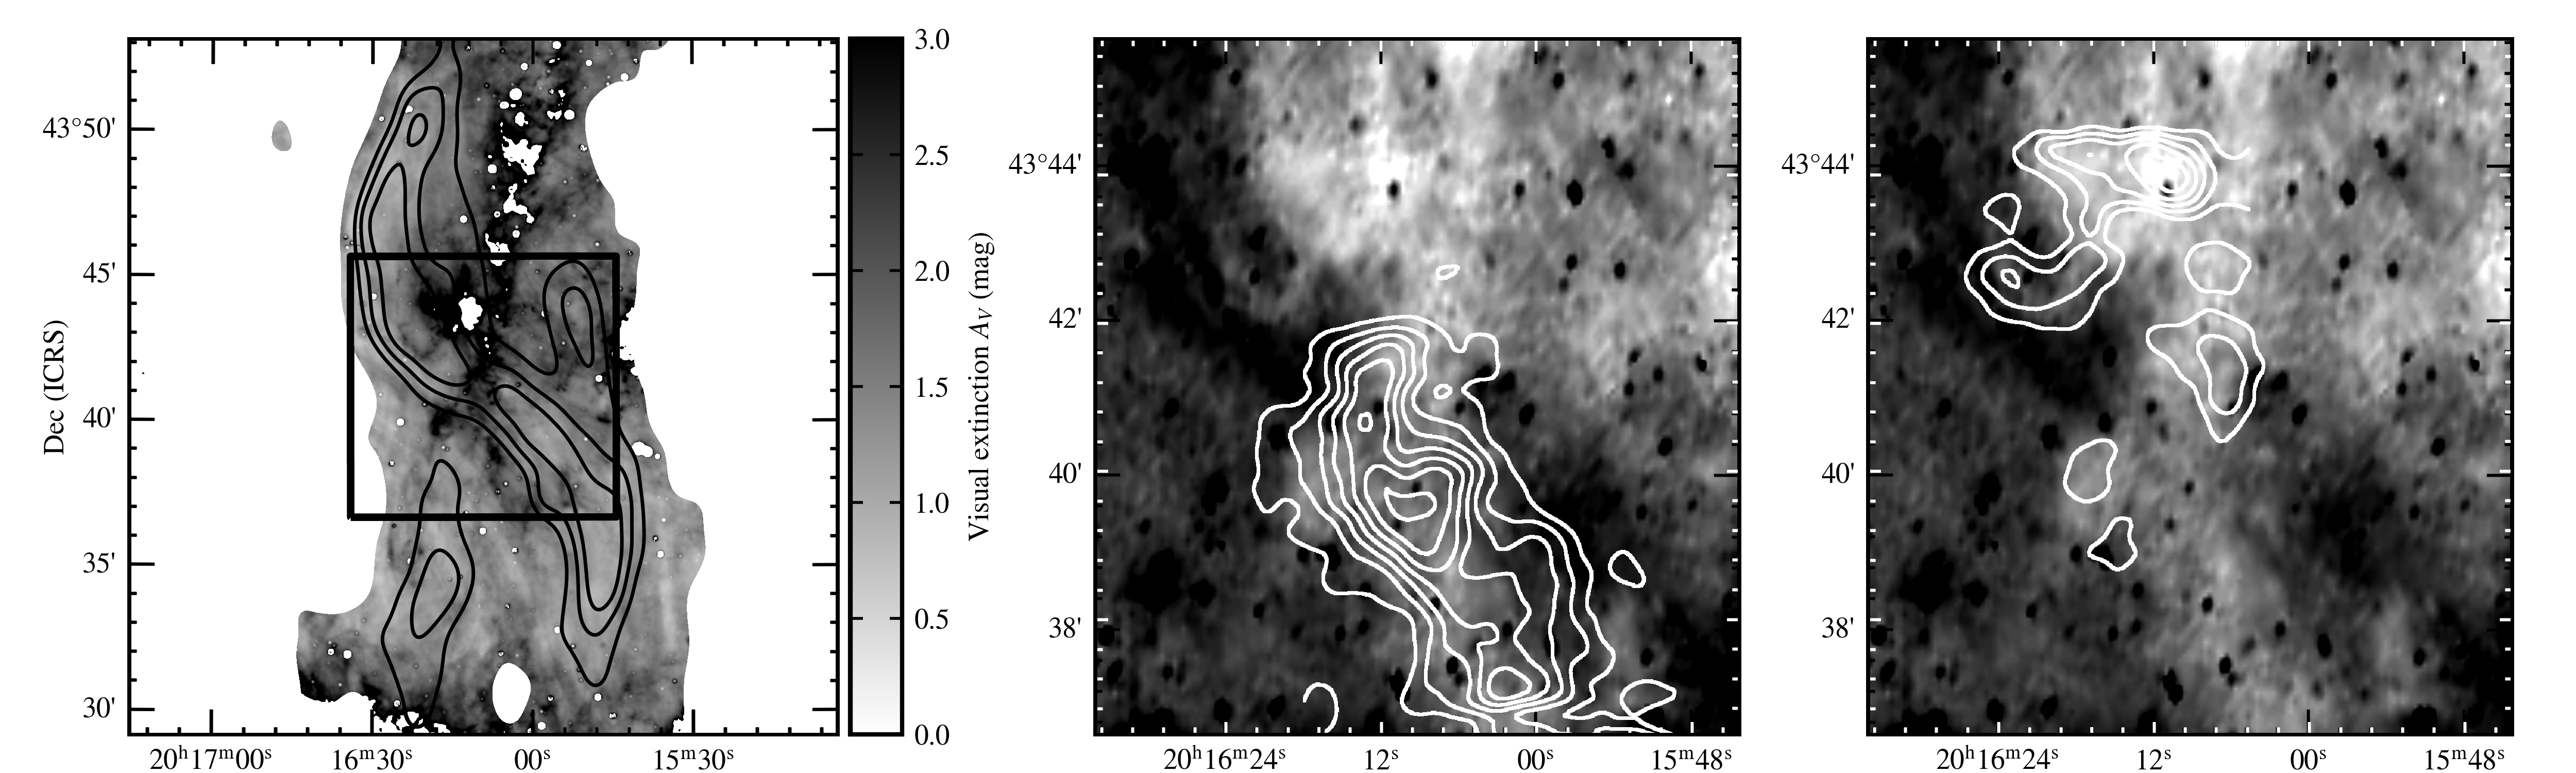
\includegraphics[width=1\textwidth]{CO_whitecont.png}
\centering
\caption{Left: extinction expressed in visual magnitudes across
  Simeis~57. For comparison, radio continuum contours
  $S_{1420} = 20,25,30\, \mathrm{mJy \, arcmin^{-2}}$ are
  superposed. Center: JCMT $^{13}$CO contours (+5 km/s component)
  superposed on the blue digital Palomar Sky Survey (DSS)
  image. Right: JCMT $^{13}$CO contours (-10 km/s component)
  superposed on blue DSS image. The right two figures are 
  a close up of the $9' \times 9'$ 
  region as indicated by the box in the extinction map.}
\label{fig:co_extinction_map}
\end{figure*}

\par \textbf{The JCMT mapping of the central clouds
  (Fig.\,\ref{fig:jcmt_co_maps}) provides the most detailed
  picture. The CO clouds closely coincide with the absorption patches
  in the visual image (Fig.\,\ref{fig:co_extinction_map}). Especially 
  the compact blue cloudlets at the same radial velocity as
  the optical nebula have clear counterparts in well-defined extinction
  patches.} The elongated red cloud coincides with the
  extinction feature extending from the nebular center to the south,
  along DWB~119. This cloud is also in front of the nebula, but given
  its different velocity, it may be at an intervening distance.

  \par \textbf{The multiple-transition CO data allow the derivation of
    the physical conditions of the molecular gas with the radiative
    transfer code RADEX \citep{vanderTak2007}}.  We assume an
  intrinsic isotopologue ratio [$^{12}$CO]/[$^{13}$CO] of 60, a carbon
  abundance C/H = 8.45 \citep[cf. ][]{arellanocrdova2020galactic}, and
  a carbon gas-phase depletion factor of a third. \textbf{The blue
    cloud core turns out to represent a relatively large column
    ($N_{H_2}\,=\,2\times10^{21}\,\mathrm{m^{-2}}$) of rather warm
    ($T_{kin}\,\geq\,30$ K) but low-density ($n_{H_2}$ = 100
    cm$^{-3}$) molecular gas which is close to the nebular gas density
    (Sect. 3.2). The dust and molecular gas of the blue cloud appears
    to be integral part of the nebula.} In contrast, the more extended
  red cloud core has a higher density ($1000\,\mathrm{cm^{-3}}$) but a
  lower column density ($\sim 1\times10^{21}\, \mathrm{cm^{-2}}$),
  with a temperature unconstrained by the observations. With standard
  gas-to-extinction ratios \citep{zhu2017_gastoextinction} \textbf{the
      extinction caused by the blue cloud is $A_{V}\,\approx\,2^{m}$
      and that caused by the red cloud $A_{V}\,\approx\,1^{m}$.  Most
      of the molecular gas and dust traced by the red CO clouds is in
      front of the nebula; a smaller amount (blue clouds) emission is
      directly associated with the nebula. There are no signs of
      embedded sources of excitation and the molecular gas column
      densities imply extinctions much too low for the obscuration of
      luminous stars}. Thus, the Simeis~57 complex is not itself
    hiding its source of excitation and we must look for it in the
    \textbf{much larger surrounding field of fragmentary molecular
      cloudlets, nebular filaments and scattered stars.}

\subsection{Stars in the Simeis~57 field}

\par From the ultraviolet and optical images in
Figs.\,\ref{fig:image_spectrum} and \ref{fig:co_extinction_map} it
might be suspected that Simeis~57 is associated with a small group of
luminous blue stars. Remarkably, several of the stars seen in the UV
images can be recognized at longer wavelengths up to $4.6\mu$m in the
near-infrared image and some can even be seen in the mid-infrared at
$12\mu$m and $22\mu$m. Because the wavelength-dependent interstellar
extinction increases steeply towards the ultraviolet, the stars in the
UV images are unlikely to suffer much extinction either locally or in
the foreground.

These stars are part of the Gaia subsample of 49 bright blue stars
whose proper motions (Fig.\,\ref{fig:gaia_figs}) suggest the presence
of two groups.  Group A (blue dots) is moving primarily west to east,
while group B (orange dots) moves primarily north to south. The
overlap between the two groups is considerable and neither group
exhibits clustering around a specific value.  The parallaxes of the
Gaia stars vary widely from 0.62 to 4.43 mas (corresponding to
distances of 225 to 1600 pc). {\bf Their} G-band extinctions {\bf are
  lower than the nebular extinction and} most of them will be stars in
  the foreground. Thus, there is no evidence that the nebula is
  physically associated with this {\bf or any other} group of stars.

\par Appendix A shows the continuum spectra of twenty prominent stars
near Simeis~57 (thirteen of which can be identified in
Fig.\,\ref{fig:image_spectrum}). As argued there, most of these stars
are ruled out as a source of excitation for Simeis~57 on grounds of
spectral type, intensity, or distance. Hence, no exciting star is
identified near the nebula either. Only the star HD 193793 = WR~140,
also known as the variable star V1687~Cyg or the spectroscopic binary
SBC9 1232 \citep{Pourbaix2004} emerges as a suitable candidate, albeit
at the large projected distance $50'$ to the east of the nebula
(cf. Fig.\,\ref{fig:Ha_mosaic}).  At the stellar distance of
1.71$\pm$0.11 kpc (\cite{smith2012}, \cite{rate2020}), this
corresponds to a projected linear separation of about 23 pc. HD 193793
consists of an evolved O4-5 star ($M_V\,=\,-6.9^{m}$) and a WC7p
Wolf-Rayet star ($M_V\,=\,-6.3^{m}$) with a combined luminosity of
more than $2\times10^6$ L$_{\odot}$ \citep{Williams2011}. It is
located in a void in the HI distribution \citep{Arnal2001} and suffers
a line-of-sight extinction $A_V\,=\,2.9$ \citep{Williams2011}. If
Simeis~57 is at the same distance as HD 193793, its gas depth as
defined by the radio emission would be $d\,=\,EM/n_e^2\,\sim\,2$
pc. 

%%%%BEGIN EDIT REFEREE
\par \textbf{In that case it covers a solid angle of $\sim0.06$
  steradian. This corresponds to blocking $0.5\%$ of the sky. Using
  the Lyman continuum photon fluxes of a WC7 star
  \citep{Crowther_2007} and those of O4I-5I stars
  \citep{Sternberg_2003} we find a combined production rate log
  $N_{Lyc}(star)\,=\, 50.03 (\mathrm{ph \, s^{-1}})$.} There appears
to be little or no absorbing gas and dust between the star and the
nebula \citep{Arnal2001}, {\bf so that an intercept rate
  $N_{lyc}(neb)\,=\,10^{47.7}\,\mathrm{ph\, s^{-1}}$ is predicted for
  the nebula.  This is practically identical to the rate derived from
  the H$\alpha$ observations in Sect. 3.3. Similarly, the intercepted
  infrared luminosity should be about $L_{TIR}\,\sim\,10^{4}$
  L$_{\odot}$. This is about five times the luminosity of the compact
  FIR source at the center of Simeis~57, and about equal to the total
  luminosity of the nebula. This is not unexpected because the patchy
  extinction and the fragmentary CO distribution seen in
  Fig.\,\ref{fig:co_extinction_map} suggests a smaller blocking factor for
  the dust clouds than for the gas.}
  
\par \textbf{The binary HD 193793 = WR140 is thus the most likely
  source for the excitation of the nebula.  In particular, the UV
  Lyman continuum output of the WR star is consistent with the strong
  [OIII] emission in the eastern half of nebula and the expected
  output of the system is in excellent agreement with the ionization
  rate implied by the observations of the nebula. }
%%%%END EDIT REFEREE
In many aspects, such as the outside location of the exciting star,
the [OIII]/H$\alpha$ emission line asymmetry, and the filamentary
appearance, Simeis~57 much resembles the California Nebula (NGC~1499)
excited by the hot runaway star $\chi$ Persei.

An investigation into the dynamics of the nebular gas might
be rewarding in studies of the region's interstellar
medium and the evolution of an early O/WC binary such as HD~193793.



\section{Conclusion}

In the previous paper on Simeis~57, \cite{israel2003} established that
the emission of the nebula is thermal, ruling out that it is a
supernova remnant. Its peculiar shape is suggestive of a rotating
outflow from either an evolving young object like an HII region or an
old evolved object like a planetary nebula. In either case, we would
expect to find a centrally located source of excitation.

This paper establishes that the nebula has a relatively low density of
about 100 cm$^{-3 }$, and suffers {\bf an extinction of not much more
  than 2$^{m}$.}  Optical spectroscopy reveals an excitation gradient
decreasing from east to west, with significant [OIII] emission east of
the main body, and very little [OIII] emission to the west. The nebula
is recognizable but not prominent in mid-infrared and far-infrared
images.  {\bf There is no major CO cloud complex but small (4-8 pc) CO
  clouds, all at $V_{LSR}\,\approx\,+5$ km s$^{-1}$, are scattered
  across the field. One of these clouds coincides with the nebula and
  also a fragmentary cloud at the nebular velocity of
  $V_{LSR}\,\approx\,-10$ km s$^{-1}$. They do not appear to be
  physically connected an both are smaller than the ionized
  nebula. They} have substantial substructure. The CO data suggest
molecular gas densities of 1000 cm$^{-3}$ and 100 cm$^{-3}$ and modest
column densities $N(H_{2})$ = 1-2 $\times$ 10$^{21}$ cm$^{-2}$. {\bf
  The CO observations clearly establish that Simeis~57 is not part of
  a larger complex but an isolated object in a larger field filled with
  fragmentary gas and dust clouds.} No luminous stars are embedded in
the dust, nor are any hidden by it; there is no central source.

The larger field surrounding the nebula reveals only one probable
excitation source. This is the evolved binary HD 193793 consisting of
an O4-5 supergiant and a WC7 Wolf-Rayet star (WR~140) at a
well-established distance of D = 1.71 kpc and with a projected
separation of 23 pc to the nebula. Both its luminosity and the
hardness of its UV radiation appear sufficient to explain the
excitation of Simeis~57. Moreover, its location to the east of the
nebula fits well with the observed [OIII] emission asymmetry. Thus, it
appears that the nebula Simeis~57 consists of separate filaments and
diffuse emission that together only fortuitously produce the
remarkably coherent appearance of an outflow object.


\begin{acknowledgements}
  We are indebted to Ardjan Sturm and Christian Groeneveld for their
  help with the May 2017 INT-WFC observations. LHTO also wishes to
  thank Ardjan Sturm for useful discussions.

\par We thank the telescope operators (TOs) of the James Clerk Maxwell
Telescope (JCMT) for conducting the observations described in this
paper. At the time, the JCMT was operated by the Joint Astronomy
Centre (JAC) in Hilo, Hawaii, on behalf of the Particle Physics and
Astronomy Research Council (P-PARC) of the United Kingdom, the Netherlands
Organization for Scientific Research (NWO), and the National Research
Council (NRC) of Canada.

\par JB acknowledges support by Funda\c{c}\~ao para a Ci\^encia e a
Technologia (FCT) through the research grants UID/FIS/04434/2019,
UIDB/04434/2020, UIDP/04434/2020 and through the Investigador FCT
Contract No. IF/01654/2014/CP1215/CT0003.

\par This work has made use of data from the European Space Agency (ESA)
mission {\it Gaia} (\url{https://www.cosmos.esa.int/gaia}), processed
by the {\it Gaia} Data Processing and Analysis Consortium (DPAC,
\url{https://www.cosmos.esa.int/web/gaia/dpac/consortium}). Funding
for the DPAC has been provided by national institutions, in particular
the institutions participating in the {\it Gaia} Multilateral
Agreement.

\par This research made use of Montage, funded by the National
Aeronautics and Space Administration's Earth Science Technology
Office, Computational Technologies Project, under Cooperative
Agreement Number NCC5-626 between NASA and the California Institute of
Technology. The code is maintained by the NASA/IPAC Infrared Science
Archive.

\par This research has made use of the SIMBAD database,
operated at CDS, Strasbourg, France 

\end{acknowledgements}

\bibliographystyle{aa}
\bibliography{pln}

\appendix
\section{Stellar neighborhood}
\par The continuum spectra of twenty relatively prominent stars near
Simeis~57, identified in Fig\,\ref{fig:bright_stars}, are shown in
Fig.\,\ref{fig:stellar_spectra}. Thirteen of these stars are also
contained in the UV-to-FIR images from
Fig.\,\ref{fig:image_spectrum}. The stellar fluxes were taken from
Simbad \citep{simbad2000}, which was accessed through the CDS portal.
Photometric measurements are mostly part of all-sky surveys. 
Catalogues and instruments included in the data are: the Sloan Digital Sky Survey
(SDSS)
\citep{Aguado2019}, the 2MASS All-Sky Catalog of Point Sources
\citep{Cutri2003}, WISE \citep{Wright2010,Jarrett2011}, Tycho-2 and the
Tycho Input Catalogue \cite{Pickles2010,Egret1992A,Ofek2008}, the MSX6C
Infrared Point Source Catalog \citep{Egan2003}, AKARI
\citep{Takita2010}, Pan-STARRS \citep{Magnier2013}, GAIA
\citep{gaiamission,gaia_data}, the  All-Sky Compiled Catalogue 
\citep{Kharchenko2009}, Hipparcos \citep{Perryman1997}, The AAVSO
Photometric All-Sky Survey (APASS) \citep{Henden2009}, the IRAS PSC/FSC
Combined Catalogue \citep{Abrahamyan2015A}, the IPHAS DR2 Source
Catalogue \citep{Barentsen2014}, the (Second-Generation) Guide Star
Catalog \citep{Lasker2008}, the Catalogue of new Herbig Ae/Be and
classical Be stars \citep{Vioque2020}, DIRBE Near-infrared Stellar Light
Curves \citep{Price2010ApJS..190..203P}, the U.S. Naval Observatory
Catalog of Positions of Infrared Stellar Sources
\citep{Hindsley1994AJ....107..280H} and Parameters and IR excesses of
Gaia DR1 stars \citep{McDonald2017MNRAS.471..770M}. 
\par For a large fraction of these stars, a few additional photometric
points with fluxes significantly below the stellar spectrum are
returned by the CDS portal. In almost all cases, these photometric
points are part of the Pan-STARRS catalogue. For the same wavelength
multiple (up to four times) photometric points are returned with
different fluxes. For each of these Pan-STARRS filters, one of the
photometric points is in line with
the stellar spectrum as indicated by other catalogues and GAIA. We have
in these cases, deleted the points that were duplicates and 
obvious errors. For two stars, the photometric points from the
IPHAS Source Catalogue were significantly below the photometric points
of other missions (at similar wavelengths) and especially below the
measurements from GAIA. Since the accuracy of GAIA for these bright
stars is higher than it is for the IPHAS catalogue, we have by hand also
removed the IPHAS datapoints in these two cases. 



\begin{figure}
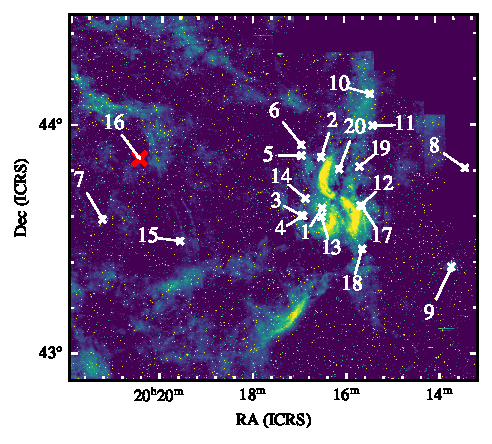
\includegraphics[width=0.48\textwidth]{Simeis_Bright_Stars.pdf}
\centering
\caption{Identification chart of bright stars near Simeis~57 for which
  continuum spectra are shown in Fig\,\ref{fig:stellar_spectra}. With 
  red (number 16, HD 193793/WR140) the spectroscopic binary SBC9 1232
  \citep{Pourbaix2004} and most likely candidate for the ionization of 
  Simeis~57 is indicated. Background map is as in Fig.
  \ref{fig:Ha_mosaic}.}
\label{fig:bright_stars}
\end{figure}

Four of these stars (Nos. 7, 16, 19, and 20) are at distances close to
the estimated distance of Simeis~57 whereas the distance of two stars
(Nos. 1 and 18) is unknown.  Stars Nos. 2, 3, 9, 10, 11, 12, 13, 15,
and 17 are all too nearby and have spectral types too late to be of
interest here.  Stars Nos. 5, 6, 8, and 14 are relatively luminous
stars of early type A0, but their output of ionizing UV photons is
still too small to matter nor are they sufficiently distant. The
spectral type of stars Nos. 1, 4, 7, 17, 18, 19, and 20 is
unknown. Star No. 17 is, however, too nearby and the IRAS PSC stars
Nos. 18 and 19, prominent in the WISE images of
Fig.\,\ref{fig:image_spectrum}, appear to be dust-embedded stars of
relatively low luminosity. This leaves for consideration stars Nos. 1,
4, 7, 16, and 20. Only star No. 16 (HD 193793) seems bright enough.
As the spectroscopic binary SBC9 1232 \citep{Pourbaix2004}, it
consists of an evolved O4/O5 star and the WC7p Wolf-Rayet star WR~140
at a distance of 1.64 kpc, with a combined luminosity of more than
$2\times10^6$ L$_{\odot}$.  \onecolumn
\begin{figure}
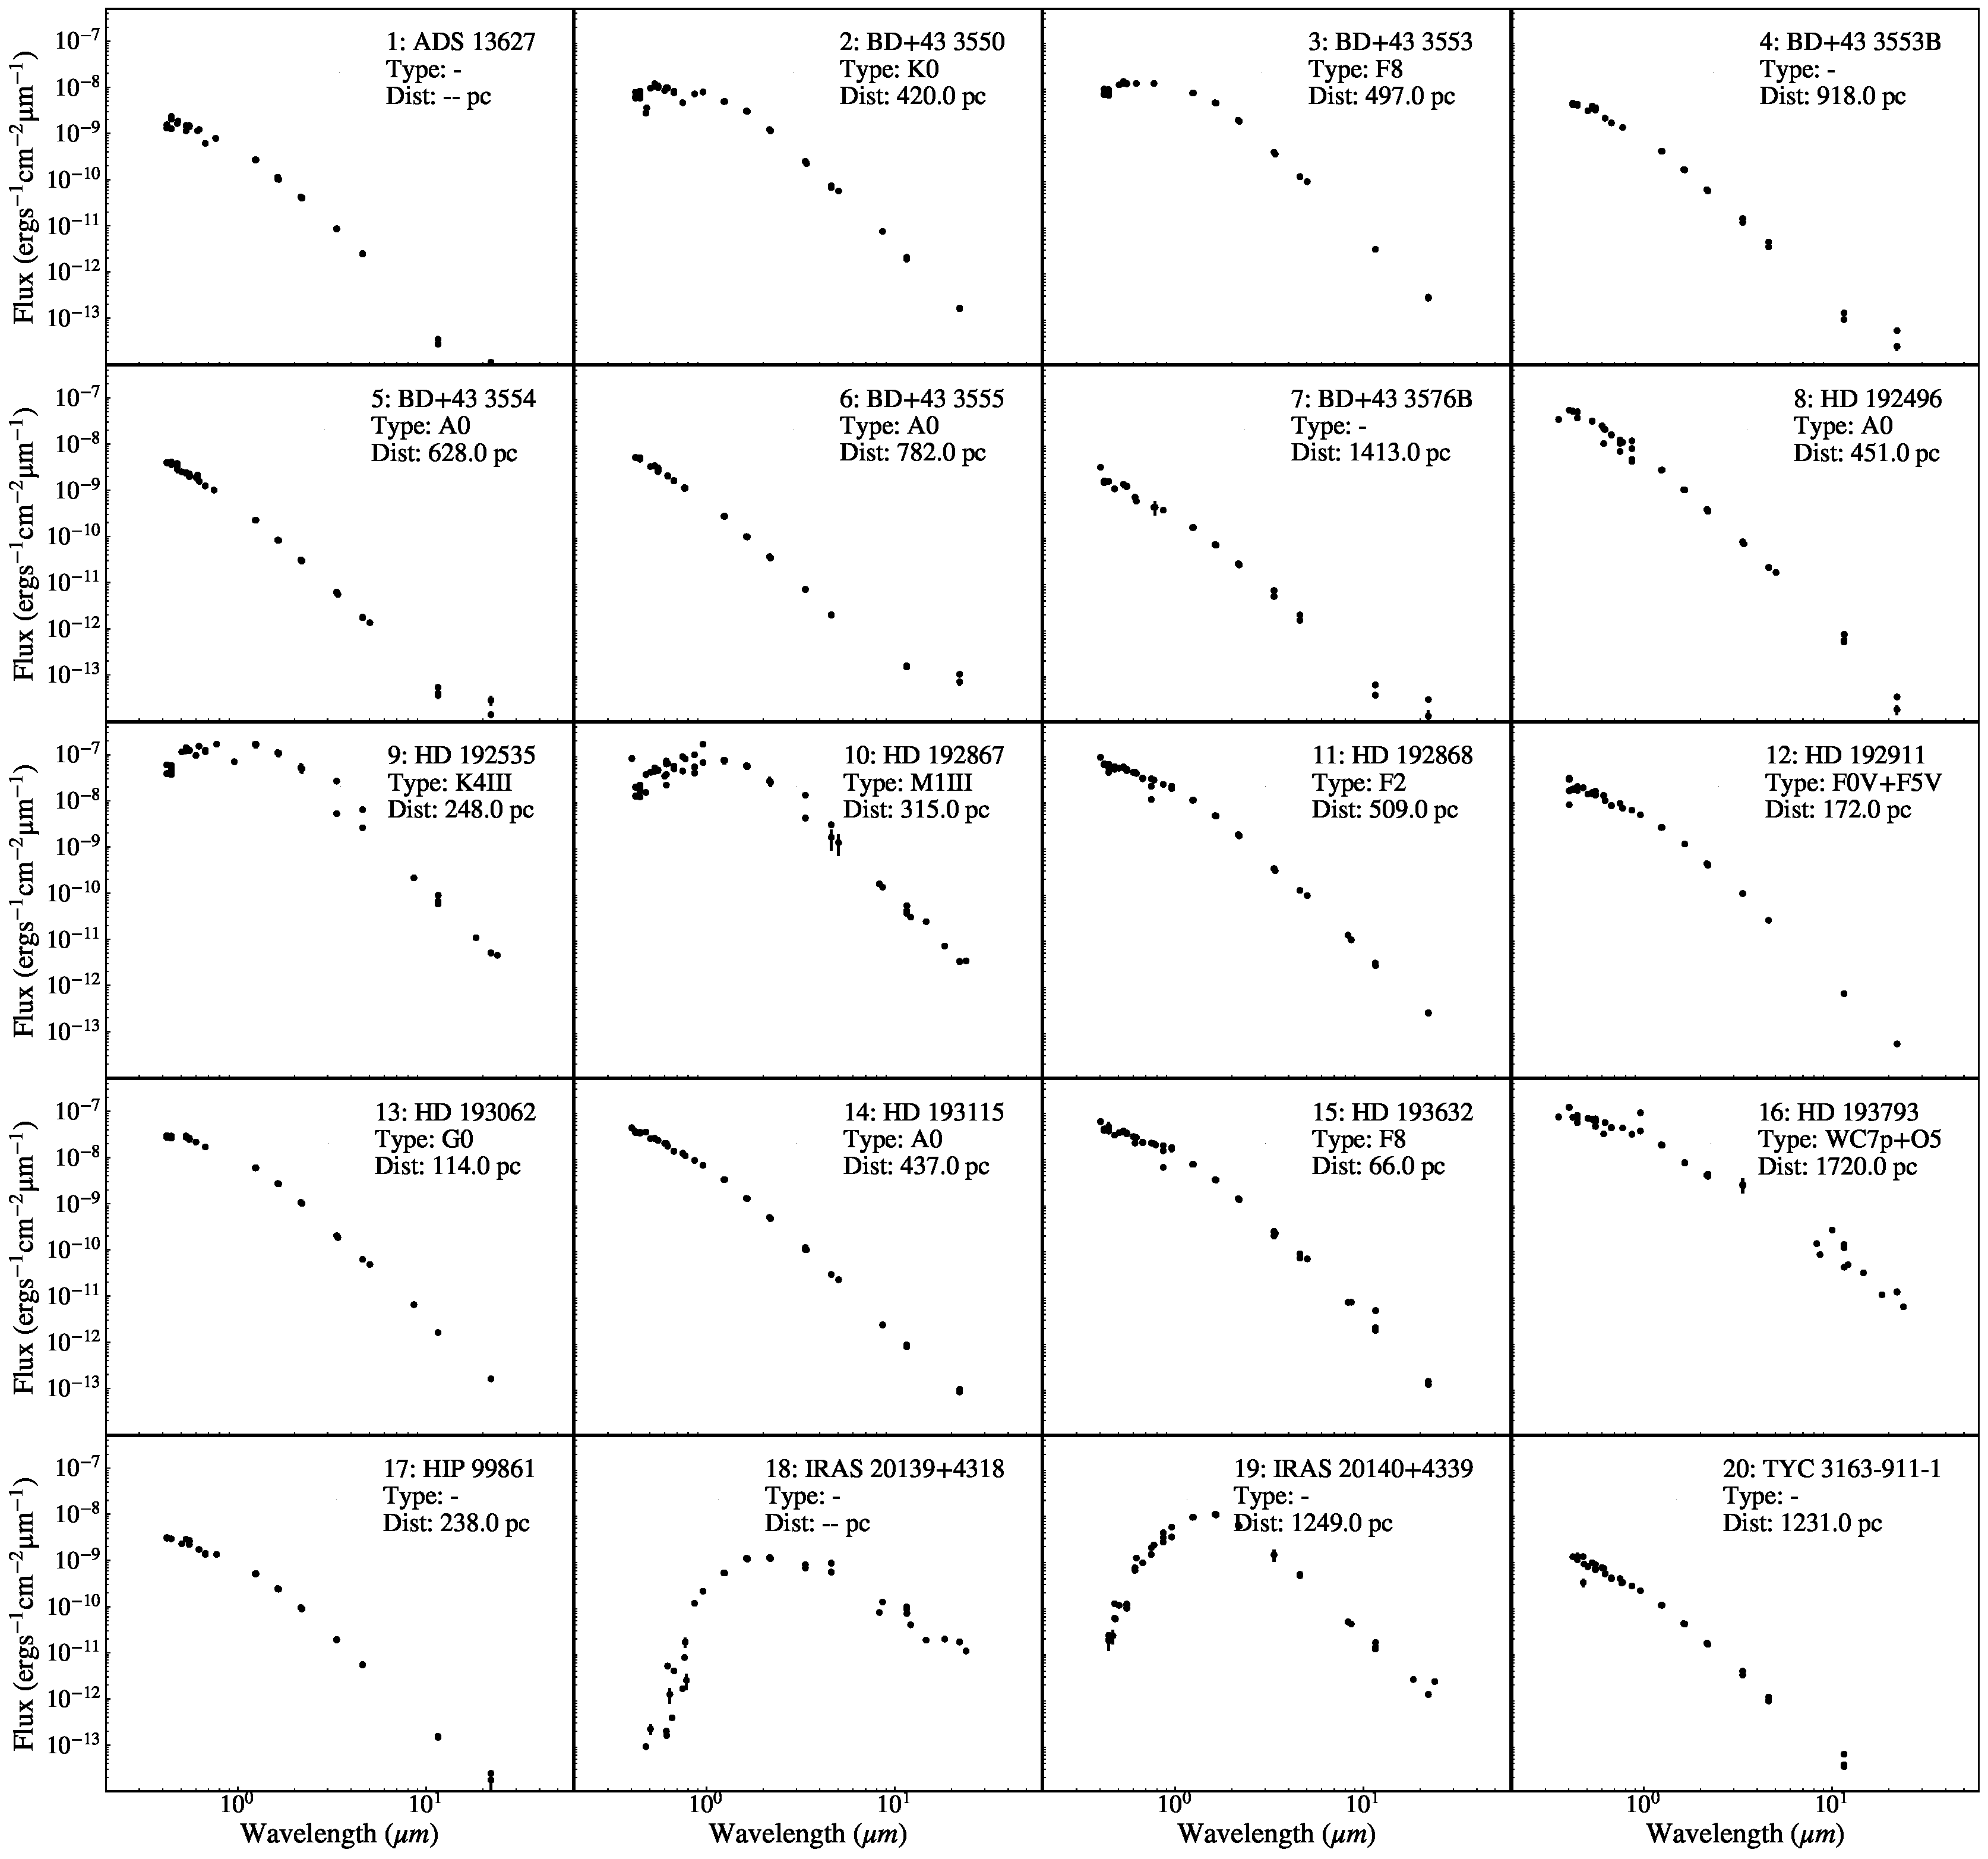
\includegraphics[width=0.98\textwidth]{stellar_spectra.pdf}
\centering
\caption{Continuum spectra of stars identified in
  Fig\,\ref{fig:bright_stars}. The distanced are as available in 
  Simbad \citep{simbad2000}}.
\label{fig:stellar_spectra}
\end{figure}



\end{document}